%%
%% Copyright 2007, 2008, 2009 Elsevier Ltd
%%
%% This file is part of the 'Elsarticle Bundle'.
%% ---------------------------------------------
%%
%% It may be distributed under the conditions of the LaTeX Project Public
%% License, either versixon 1.2 of this license or (at your option) any
%% later version.  The latest version of this license is in
%%    http://www.latex-project.org/lppl.txt
%% and version 1.2 or later is part of all distributions of LaTeX
%% version 1999/12/01 or later c.
%%
%% The list of all files belonging to the 'Elsarticle Bundle' is
%% given in the file `manifest.txt'.
%%

%% Template article for Elsevier's document class `elsarticle'
%% with harvard style bibliographic references
%% SP 2008/03/01
%%
%%
%%
%% $Id: elsarticle-template-harv.tex 4 2009-10-24 08:22:58Z rishi $
%%
%%
\documentclass[preprint,authoryear,12pt]{elsarticle}

%% Use the option review to obtain double line spacing
%% \documentclass[authoryear,preprint,review,12pt]{elsarticle}

%% Use the options 1p,twocolumn; 3p; 3p,twocolumn; 5p; or 5p,twocolumn
%% for a journal layout:
%% \documentclass[final,authoryear,1p,times]{elsarticle}
%% \documentclass[final,authoryear,1p,times,twocolumn]{elsarticle}
%% \documentclass[final,authoryear,3p,times]{elsarticle}
%% \documentclass[final,authoryear,3p,times,twocolumn]{elsarticle}
%% \documentclass[final,authoryear,5p,times]{elsarticle}
%% \documentclass[final,authoryear,5p,times,twocolumn]{elsarticle}

%% if you use PostScript figures in your article
%% use the graphics package for simple commands
%% \usepackage{graphics}
%\usepackage{cases}
%% or use the graphicx package for more complicated commands
\usepackage{graphicx}
%% or use the epsfig package if you prefer to use the old commands
\usepackage{epsfig}

\usepackage{comment}
\usepackage{epstopdf}
\usepackage{bm}
\usepackage{hyperref}
\hypersetup{colorlinks=true, urlcolor=blue, linkcolor=blue, citecolor=red}

%% The amssymb package provides various useful mathematical symbols
\usepackage{amssymb,amsmath}
%% The amsthm package provides extended theorem environments
%% \usepackage{amsthm}

%% The lineno packages adds line numbers. Start line numbering with
%% \begin{linenumbers}, end it with \end{linenumbers}. Or switch it on
%% for the whole article with \linenumbers after \end{frontmatter}.
%% \usepackage{lineno}

%% natbib.sty is loaded by default. However, natbib options can be
%% provided with \biboptions{...} command. Following options are
%% valid:

%%   round  -  round parentheses are used (default)
%%   square -  square brackets are used   [option]
%%   curly  -  curly braces are used      {option}
%%   angle  -  angle brackets are used    <option>
%%   semicolon  -  multiple citations separated by semi-colon (default)
%%   colon  - same as semicolon, an earlier confusion
%%   comma  -  separated by comma
%%   authoryear - selects author-year citations (default)
%%   numbers-  selects numerical citations
%%   super  -  numerical citations as superscripts
%%   sort   -  sorts multiple citations according to order in ref. list
%%   sort&compress   -  like sort, but also compresses numerical citations
%%   compress - compresses without sorting
%%   longnamesfirst  -  makes first citation full author list
%%
%% \biboptions{longnamesfirst,comma}

% \biboptions{}
\newcommand{\PN}[2][error]{P$_{#1}$DG-P$_{#2}$}


\journal{Computer Methods in Applied Mechanics and Engineering}

\begin{document}

\begin{frontmatter}

%% Title, authors and addresses

%% use the tnoteref command within \title for footnotes;
%% use the tnotetext command for the associated footnote;
%% use the fnref command within \author or \address for footnotes;
%% use the fntext command for the associated footnote;
%% use the corref command within \author for corresponding author footnotes;
%% use the cortext command for the associated footnote;
%% use the ead command for the email address,
%% and the form \ead[url] for the home page:
%%
%% \title{Title\tnoteref{label1}}
%% \tnotetext[label1]{}
%% \author{Name\corref{cor1}\fnref{label2}}
%% \ead{email address}
%% \ead[url]{home page}
%% \fntext[label2]{}
%% \cortext[cor1]{}
%% \address{Address\fnref{label3}}
%% \fntext[label3]{}

\title{The Overlapping Control Volume Finite Element Method for Multi-Phase Porous Media Flow Modelling \\
Part II: Applications}

\author[IC]{D. Pavlidis}\corref{cor1}\ead{dimitrios.pavlidis@imperial.ac.uk} \author[UoA]{J.L.M.A. Gomes}  \author[IC]{J.R. Percival} \author[IC]{P. Mostaghimi} \author[IC]{P. Salinas} \author[IC]{Z. Xie} \author[IC]{C.C. Pain} \author[IC]{M. D. Jackson}
\author[IC]{M. Blunt} 
\cortext[cor1]{Corresponding author.}

\address[IC]{Applied Modelling and Computation Group, Department of Earth Science and Engineering, Imperial College London, UK}
\address[UoA]{Environmental $\&$ Industrial Fluids Mechanics Group, School of Engineering, University of Aberdeen, UK}

\begin{abstract} 
This paper is the second part of a two-part paper on a novel finite
element method FEM-based formulation for simulating multi-phase flows
through porous media. In the first paper, the formulation, based upon
the overlapping control volume finite element method, was developed
and, simple validation test-cases were presented. In this second
paper, the OCVFEM formulation is applied to a set of multi-phase
porous media flows test-cases to assess the performance and numerical
accuracy of continuous and discontinuous (between elements) element
pairs.  The test cases include structured and unstructured (triangular
/ tetrahedral) meshes, as well as heterogeneous problems with large
permeability ratios. Numerical solutions are in good agreement with
(semi-)analytically obtained data.
\end{abstract}

\begin{keyword}
%% keywords here, in the form: keyword \sep keyword
Multi-phase porous media flow \sep overlapping control volume finite element method. 
\end{keyword}

\end{frontmatter}

%\tableofcontents
% \linenumbers
%%%                   %%%
%%%      SECTION      %%%
%%%                   %%%
\section{Introduction}


This is the second part of a two part paper developing and applying
novel computational methods for multi-phase flow in porous media. The
new overlapping control volume finite element method was introduced in
the first part of this paper \citep{gomes_2013}.

This paper focuses on exploring, by numerical simulations of
multi-phase flow in porous media, the fidelity of the results yielded
by the continuous pressure (\PN[n]{n+1}) and discontinuous pressure
(P$_n$DG-P$_n$DG and P$_{n+1}$DG-P$_n$DG) families of finite element
(FE) types introduced in the first paper. By presenting numerical
experiments in 1-, 2- and 3-D, we shall study the accuracy, reliability
and convergence rates yielded from the proposed FE
families for modelling multi-phase displacements in porous media. In this
way, quadratic and linear elements are tested for different
geometries, meshes and permeability fields. The methods show in all
cases good behaviour and a veracious representation of the fluid flow.

The remainder of this paper is organised as follows. A brief
description of the model is given in
Section~\ref{Section:SummaryPaper1} followed by the model validation
against analytical solutions of the classical Buckley-Levrett
problem. In Section~\ref{res2}, water-flood problems (i.e., immiscible
fluids displacement) are simulated in 2-D to assess the flow
behaviour in heterogeneous porous media. The impact of
large permeability ratios (i.e., highly heterogeneous porous matrix)
in the model is investigated in Sections~\ref{res3}, \ref{res4}
and~\ref{res5}. Additionally, in Section~\ref{res4} the model
performance when elements are skewed due to large domain aspect ratio
is investigated. A brief summary of the results are presented in
Section~\ref{conc} followed by many conclusions drawn from the two
inter-linked papers.


%\setlength\parindent{0pt}


%\section{Model Validation}\label{Section:Results}
\section{Summary of the Model Formulation}\label{Section:SummaryPaper1}
The extended Darcy's law and phase saturation equations for $N_{p}$
immiscible fluid phases can be expressed as:
\begin{equation}
  \underline{\underline{\sigma}}_{\alpha} \mathbf{u}_{\alpha} :=
  S_{\alpha}\left(\displaystyle\frac{\mathbf{K}
    \mathcal{K}_{r_\alpha}}{\mu_{\alpha}}\right)^{-1}\mathbf{u}_{\alpha}=
  -\nabla p + \mathbf{s}_{u_\alpha},
  \label{Darcy}
\end{equation}
\begin{equation}\label{Eqn:Saturation}
  \phi\displaystyle\frac{\partial S_{\alpha} }{\partial t} + \nabla
  \cdot \left( {\mathbf u}_{\alpha} S_{\alpha}\right) =
  s_{\mbox{cty}_\alpha},
\end{equation}
where $\alpha\in\left[1,N_{p}\right]$ is the phase index, $S_\alpha$,
$\mathcal{K}_{r_\alpha}$ and $\mu_\alpha$ are phase saturation,
relative permeability and viscosity, respectively. The quantity
$\underline{\underline{\sigma}}_{\alpha}$ represents the
transmissibility of the phase. The vector $\mathbf{u_\alpha}$ is the
saturation-weighted Darcy velocity and the vector
$\mathbf{s}_{u_\alpha}$ is a source, containing terms such as gravity
forces and capillary pressure, associated with the force balance. Here
$\mathbf{K}$ is the medium absolute permeability tensor, $\phi$ is the
rock porosity and $p$ is the pressure, assumed independent of
phase. The mass source term $s_{\mbox{cty}_\alpha}$ may for example be
used to model the exchange of saturation between phases.

The overlapping control volume finite element method discretisation
was introduced in part I of this paper \citep{gomes_2013}. Pressure
is represented by finite element basis functions on a given FE mesh
partition, with the absolute permeability tensor assumed element-wise
constant on the same mesh. Saturation is represented by flat functions
on the node-centred CV space dual to the finite element
mesh. Velocities are represented by finite element basis functions
with support on the spaces formed by the intersection between the
saturation CV's and pressure FE's.

The weak form discretised force balance equations for time level $n$
and phase $\alpha$ are thus of the form:
\begin{eqnarray} 
  %\sum\limits_{E}\int_{\Omega_E} { {Q}}_i \left({\underline {\underline \sigma}}_k^{n+1} \cdot  {\mathbf u}^{n+1} + \nabla p^{n+1} -{\mathbf s}_u^{n+1} \right) dV +  \displaystyle\frac{1}{2} \oint_{\Gamma_{E}}  {Q}_i {\mathbf n} \left(p^{n+1} - p_{nab^{n+1}}\right) d\Gamma + \nonumber \\
  \left. \int\limits_{\Omega} { {Q}}_i \left({\underline {\underline \sigma}}_\alpha^{n}  {\mathbf u}^{n}_\alpha + \nabla p^{n} -{\mathbf s}_{u_\alpha}^{n} \right) dV \right. +  \oint_{\Gamma_{E}}  {Q}_i {\mathbf n} \left(p^{n} - \tilde{p}^{n}\right) d\Gamma  \nonumber \\
  + \oint_{\Gamma_{\Omega p}} { Q}_i {\mathbf n} \left(p^{n} - p_{bc}^{n}\right) d\Gamma &=& \bm{0},
  \label{force-semi-disc} 
\end{eqnarray} 
where the finite element pressure and velocity fields are given by:
\begin{displaymath}
p^{n}:=p(\bm{r},t)=\sum\limits_{j=1}^{\mathcal{N}_p} P_{j}(\bm{r}) p_{j}^{n} \;\;\text{  and  }\;\; {\bf u}_\alpha^{n}:=\bm{u} (\bm{r},t) =\sum\limits_{j=1}^{\mathcal{N}_u} Q_{j}(\bm{r}){\bf u}_{\alpha,j}^{n},
\end{displaymath} 
in which $\bf {n}$ is the normal to the element, $\mathcal{N}_{p}$ and
$\mathcal{N}_{u}$ are the number of degrees of freedom for the FE
pressure and velocity representations, respectively. Here $\Omega$
is the volume domain with $\Omega_E$ the subspace associated with
velocity element $E$, $\Gamma_{E}$ is the interior surface boundary of
the element $E$ and $\Gamma_{\Omega p}$ is the boundary of the domain
on which pressure is set weakly to $p_{bc}$. The inter-element
pressure, defined by:
\[\tilde{p}=\lim_{\delta\rightarrow 0}(p(\bm{r}+\delta \mathbf{n})+p(\bm{r}-\delta \mathbf{n}))/2\] is the average of the finite element pressures on either side of the boundary of element $E$. 

The saturation equations (Eqn.~\ref{Eqn:Saturation}) are discretised
in space by testing them with CV basis functions and in
time with the $\theta$-method, in which $\theta=0.5$ is used as much
as possible as discussed in part I of this paper. The resulting
equations for time step size $\Delta t$ and phase $\alpha$ are given
by:
\begin{eqnarray}
  \displaystyle \int_{\Omega} M_{i}
  \left(\frac{S_{\alpha,i}^{n+1}-S_{\alpha,i}^{n}}{\Delta t}\right) dV +  \nonumber \\
  \displaystyle \oint_{ {\Gamma_{CV}}_{i}} \left ( \theta \mathbf{n}
  \cdot \mathbf{u}_{\alpha}^{n+1} S_{\alpha}^{n+1} + (1-\theta)
  \mathbf{n} \cdot \mathbf{u}_{\alpha}^{n} S_{\alpha}^{n} \right)
  d\Gamma -\displaystyle \int_{\Omega} M_{i}
  s_{cty,\alpha}^{n+\theta} dV &=& 0,
  \label{detail-global-cty}
\end{eqnarray}
where $S^{n}_{\alpha,j}:=S(\bm{r},t)=
\sum_{j=1}^{\mathcal{N}_p} M_j(\bm{r}) S^n_{\alpha,j}$. The system is
closed by the conservation constraint, $\sum_\alpha S_\alpha=1$.  A
set of coupled equations for pressure and velocity are obtained from
the overlapping CVFEM-based discretised Darcy equations
(Eqn.~\ref{force-semi-disc}) and by the sum, over all phases, of the CV-based
saturation equations (Eqn.~\ref{detail-global-cty}).

%At time level $n+1$, the coupled multiphase Darcy and global mass conservation are represented, in matricial form, as
%\begin{equation}
%\begin{cases}
%\mathbf{M}_{\sigma} \underline{\bf u}^{n+1} = \mathbf{C}\underline{\bf p}^{n+1} + \underline{\bf s}_{u}^{n+1} \\
%\mathbf{M}_{p} \underline{\bf p}^{n+1} + \mathbf{B}^{T} \underline{\bf u}^{n+1} = \underline{\bf s}_{p}^{n+1}
%\end{cases}
%\end{equation}

\section{Classical Buckley-Leverett Test-Cases}\label{classical_BL}

In this section, the Buckley-Leverett \citep{buckley1942} 
problem is modelled with phase 1 $\left(S_{l}=1\right)$ being injected 
at a constant velocity $u_{1}=1$ into a porous medium saturated by 
phase 2 $(S_{2}=1,$ $\phi=0.5)$.  

Relative permeability in this paper is calculated as a quadratic 
function of saturation with residual saturation of phase 1 and 2  $S_{1}=0.1$ 
and $S_{2}=0.3$ ,respectively.  The endpoint of the relative permeabilities
 of phases 1 and 2 are 0.8 and 0.3, respectively (see Table 1).

The length of the domain is 4
non-dimensional units. On the outlet boundary condition, the pressure
level is set to zero and all remaining boundary conditions are weakly
applied.

Despite the one-dimensional nature of the problem, 2- and 3-D
simulations were performed using structured and unstructured meshes to
evaluate the multi-dimensional capabilities of the model.

 All simulations used the overlapping mixed-DGFEM with \PN[0]{1},
 \PN[1]{2} and/or \PN[2]{3} element-pairs with continuous /
 discontinuous (between elements) formulations with saturation
 collocated at pressure nodes. Although saturation is calculated using
 a CV formulation, a FEM interpolation is used to form the high-order
 fluxes and these are also used for most of the plots. In all 1-D
 simulations, mesh grids were designed with equi-sized elements,
 whilst 2-D meshes were regular, structured and one-element wide with
 unity aspect ratio. The width of the 2-D numerical domain is
 inversely proportional to the number of elements. The time-step size
 varied linearly within 0.125-3.125$\times$10$^{-3}$ seconds range for
 1-D simulations, and a fixed time-step of 1.0$\times$10$^{-4}$ for
 all 2- and 3-D simulations.

%\begin{comment}
%\subsection{Continuous Formulation}
%\paragraph{Upwind Solution} 
%In Fig.~\ref{bl-exact-meth-upwind} the CV solution of the water-phase saturation and equivalent quadratic FEM interpolation are presented (\PN[1]{2}). As it can be seen, the solution converges with increased resolution. Notice that the corners of the CVs are very close to the converged solution. This can be explained as the velocities are upwinded (and also the relative permeabilities), and at these corners the equations reach the balance necessary to match the analytical solution.
%\end{comment}

\paragraph{Convergence Analysis}
Convergence analyses were performed for the 1- and 2-D problems with a
number of (regular) mesh resolution and element pairs. The time-step
size was linearly varied from 1.25$\times$10$^{-4}$ to
3.25$\times$10$^{-3}$ seconds. Figure~\ref{fig:BL_profiles} shows
phase 1 saturation profiles at time $t=0.5$ for mesh grids varying
from 5 to 500 elements, and for different element types -- \PN[0]{1},
\PN[1]{2} and \PN[2]{3} (the geometry symmetry line is used to extract
data from the 2-D simulations).  In general, results are in good
agreement with the analytic solution for all resolutions and
element-pairs however, for coarser meshes, high-order elements-pairs
(\PN[2]{3} for 1-D using 5 elements and \PN[1]{2} for 2-D using 20
elements) perform significantly better and are able to capture the
sharp-front more accurately. As far as the 2-D simulations are
concerned, the coarse mesh simulation performs slightly worse than its
1-D counterpart but for higher resolutions, results are identical.

These conclusions become clearer in Fig.~\ref{fig:BL_converg-rates},
where convergence rates are shown. The L1 and L2 errors are defined
as,
\begin{displaymath}
  \displaystyle\frac{\sum\limits_{i=1}^{N}\left|S_{i}^{\text{simulated}}
    - S_{i}^{\text{analytical}}\right|}{N}\;\;\text{ and }\;\;
  \displaystyle\frac{\sqrt{
      \sum\limits_{i=1}^{N}{\left(S_{i}^{\text{simulated}} -
        S_{i}^{\text{analytical}}\right)^{2}}}}{N},
\end{displaymath}
respectively, where $S_i$ is the saturation of phase 1 at the $i$-th
node point. In addition, convergence rates for simulations performed
with full upwinding scheme are shown.


%\paragraph{Optimal Upwinding} 
%In order to optimise the upwind formulation (Section~\ref{FluxLimitingSection}), we investigated a 80/20$\%$ up/downwinding ratio -- Fig.~\ref{bl-exact-meth-cv-0-8-ele50}, with good agreement with the converged solution. 
%The optimal solution for 50 elements using optimal upwinding, as described in 
%part I, is shown in Fig.~\ref{bl-exact-meth-cv-0-8-ele50}, with a rapid convergence. For these simulations there are no oscillations in the corresponding CV solutions -- the FEM interpolation (using Galerkin projection) of the CV solution, however it does show, as expected, oscillatory behaviour near the shock-fronts. 

\subsection{Discontinuous Formulation}
In this section, results for the fully discontinuous formulation are
presented. Discontinuity of the pressure field between elements allows
the use of coarse meshes to represent abrupt changes in the
solution. Figure~\ref{bl-dg-2eles} shows converged CV phase 1
saturation solutions and the corresponding FEM interpolated
solutions. This solution was obtained with upwinding within and
between the elements.  Convergence rates for the test-cases performed
with the fully discontinuous formulation (between elements) are shown
in Fig.~\ref{fig:BL_converg-rates_DG}.

Solutions obtained with upwinding and central difference schemes are
shown in Fig.~\ref{bl-dg-cent-4-10-20} for different resolutions, and
compared against the continuous (converged) solution with good
agreement. In this plot, one can also note the suppression of
oscillations resulting from the upwinding scheme.

In Figure~\ref{bl-dg-4-10-vers-cty}, saturation solutions obtained
using first (P$_{1}$) and second-order (P$_{2}$) functions in the FE
representation of pressure are shown both for continuous and
discontinuous representations. At coarse resolution the discontinuous
solution is more accurate. By comparing P$_{1}$ and P$_{2}$ solutions
in pressure, we demonstrate that near the shock-front there is little
benefit in using high-order discontinuous elements, thus linear
elements perform well compared to quadratic elements.

\subsection{2- and 3-D Simulations}
Following the convergence analysis, a number of numerical experiments
were performed to assess the robustness of the method in fully
unstructured meshes. Phase 1 saturation surface maps (and the
corresponding meshes) for 2- and 3-D simulations at time $t=0.5$ are
shown in Fig.~\ref{fig:maps2d_3d}. The simulations presented in this
section were performed using the \PN[1]{2} element-pair in fully
unstructured mesh-grid.

Saturation profiles for the phase 1 at time $t=0.5$ are shown in
Fig.~\ref{fig:BL_2d_profiles}. Results are not spatially averaged and
the geometry symmetry line is used to extract data for all
simulations. The structured coarse mesh uses $1 \times 19$ layers in
the lateral and flow directions, respectively. The structured medium
mesh uses $3 \times 40$ layers. The solution field converged towards
the analytical solution with the increase of the mesh resolution;
additionally, no substantial improvement was observed when structured
and unstructured \PN[1]{2} mesh were used. However, the use of
unstructured mesh (and potentially higher-order triangle and
tetrahedra elements) is advantageous for flow simulation in complex
geometries as demonstrated by \cite{jackson_2013}.


\section{Immiscible Displacement in Heterogeneous Porous Media}\label{res2}
%\section{A 4-region modified Buckley-Leverett test case}
This test case was designed to demonstrate the numerical robustness of
the method when solving multi-fluid flow problems involving
heterogeneous porous media.  Here, phase 1 is injected in a fully
saturated $\left(S_{2}=1\right)$ 2-D square porous matrix domain of
side length one and uniform porosity $\left(\phi=0.5\right)$ --
Fig. \ref{fig:4reg_BL_schematic}. However, unlike the test-cases in
Section \ref{classical_BL}, the permeability field is not uniform and
four equally sized $\lq$regions' are designed.  Permeability fields in
regions R1 and R4 are 4 times larger than that of regions R2 and R3,
i.e.,
\begin{displaymath}
  \mathbf{K}^{\text(1)}=\mathbf{K}^{\text(4)} =
  4\mathbf{K}^{\text(2)}=4\mathbf{K}^{\text{(3)}}.
\end{displaymath}
Phase 1 is uniformly injected at a velocity of $u_{l}=1$ on the left
boundary to displace the oil in the porous domain. On the outflow
boundary the pressure level is set to zero. Free-slip boundary
conditions are applied on the sides of the domain for the two velocity
fields. All boundary conditions are applied weakly. For relative
permeability calculations $\left(\mathcal{K}_{rk}\right)$, the
irreducible phase 1 and residual phase 2 saturations are set to 0.1
and 0.2, respectively; the endpoint of phase 2 and phase 1 relative
permeabilities are 0.3 and 0.8, while the Corey exponent is assumed as
2.

Two sets of simulations are performed using coarse (402 elements with
2412 nodes) and fine (3714 elements with 22284 nodes) meshes; in the
first set (A) the overlapping mixed DGFEM and the \PN[1]{2}
element-pairs are used, with time-step sizes of 1$\times$10$^{-3}$ and
5$\times$10$^{-4}$ seconds for simulations performed with coarse and
fine meshes, respectively. In the second set of experiments (B)
\PN[2]{2}DG element-pairs are used, with time-step sizes of
5$\times$10$^{-4}$ and 1$\times$10$^{-4}$ seconds for coarse and fine
meshes.

Figure~\ref{fig:4reg_maps} shows the phase 1 saturation profile maps
(at time $t=0.08$ seconds) for all four simulations. The results
yielded by the experiment (A) are depicted in the top left, coarse
mesh, and top right, fine mesh. The results obtained from experiment
(B) located on the bottom left, coarse mesh, and bottom right, fine
mesh. A laboratory experiment with similar setup was performed by
\citet{dawe_2008} to investigate miscible and immiscible displacement
in heterogeneous permeability and wettability cases.

For the immiscible displacement, phase 1 was uniformly injected from
the left-hand side boundary (injection rate of $\sim$1 ml/min in a
domain of 20$\times$10$\times$0.6 cm, glass ballotini beads produced
porosity of 0.4, and permeability ratio of 2.5). Snapshots in
Fig.~\ref{fig:4reg_maps} show the phase 1 flood $\lq$fingering' across
the central regions (R1 $\Rightarrow$ R4) demonstrating the
preferential flow through highly permeable matrix. This is in good
qualitative agreement with the laboratory experiments \citep[see
  Figs. 5 and 6 in][]{dawe_2008}.


Figure~\ref{fig:4reg_plots} shows phase 1 saturation profiles (at time
$t=0.08$ seconds) for all simulations. Comparing the results obtained
by both sets of experiments, a better agreement between the results
yielded by the simulations (B) -- i.e., with \PN[2]{2}DG
element-pairs, can also be observed.


\section{Underground Caisson}\label{res3}
Numerical models may fail when a high permeability gradient is in the
domain by introducing fluid in the low-permeability region not due to
a physical phenomena, but because of numerical dispersion. Thus, the
purpose of this numerical experiment is to test the fluid flow
behaviour across two distinct porous media characterised by high
different permeabilities.

The considered domain is characterised by a low-permeability square
region, with dimensions of 0.5 $\times$ 0.5 unit-area, which is
embedded in a high-permeability region with dimension 1 $\times$
1. The porosity of the whole domain and the permeability of the
high-permeability region are of 0.5 and 10$^{4}$ respectively. The
necessary parameters to obtain the relative permeability
$\left(\mathcal{K}_{rk}\right)$ are the following: the irreducible
phase 1 and residual phase 2 saturations are $S_{wi} = 0.1$ and
$S_{orw}=0.3$, respectively; Corey exponent is $N=2$; the endpoint of
phase 2 and phase 1 relative permeabilities are 0.3 and 0.8.

Regarding the initial state and the boundary conditions of the
experiment, at rest state the domain is fully saturated of phase 2
($S_o=1$). Next, phase 1 is injected with a constant velocity of
$(1,0)$ through the left boundary that can exit only through the right
boundary, which have a constant pressure of zero.

Two sets of numerical experiments are performed, one uses the
\PN[0]{1} element pair and a time step of 5$\times$10$^{-3}$ and the
second experiment the \PN[1]{1}DG element-pair and a time step of
1$\times$10$^{-4}$. Both use the same mesh and the same permeability
map, see Fig.~\ref{fig:square_permeability} (top).

Figure~\ref{fig:square_permeability} displays snapshots of phase 1
saturation profile at $t = 0.15$ and $t = 0.5$ for both
simulations. The simulation performed with \PN[0]{1} elements presents
a small dispersion of phase 1 into the low-permeability region,
whereas the saturation profile in the \PN[1]{1}DG simulation presents
a defined frontier between the low-permeability region and the
high-permeability area. Despite this small difference, both
experiments are in good agreement and provide satisfactory results by
making the fluid to go around the low-permeability region.

\section{High-Permeability Wedge-Shaped Region}\label{res4}
Fractures and cracks in porous media are ubiquitous, however, they are
not easy to model due to they small size. However, cracks may have a
dramatic impact in the behaviour of the flow since they can act as
conducts with a very high permeability. Usually, they are
characterised by thin tip and a high permeability. In order to test
the behaviour of the model presented in this paper, in the present
numerical experiment consists in a wedge-shaped high-permeability
region embedded in a rectangular low-permeability (permeability ratio
of 100) domain. The permeability map is shown in
Fig.~\ref{fig:wedge_permeability}.

Three different experiments were performed, two using the \PN[0]{1}
element-pair and one using the \PN[2]{1}DG element-pair. For the first
experiment using the \PN[0]{1} element-pair, the mesh is composed of
56902 elements, whereas for the second experiment the mesh is composed
of 672 elements. For the \PN[2]{1}DG element-pair example this latter
mesh is considered as well. The non-dimensional rectangular domain is
1 $\times$ 0.1 and the wedge is defined by a high of 0.025 and a slope
of $1/30$. The porosity is uniform and equal to 0.5. The irreducible
water and residual oil saturations are set to zero. Initially, the
porous media is fully saturated with an incompressible fluid
$\left(S_{2}=1\right)$. An immiscible fluid is injected from the left
boundary with a constant pressure of 1 and a saturation of
$S_{1}=1$. On the outflow boundary, the pressure level is set to zero.

Free-slip boundary conditions are applied on the sides of the domain
for the two velocity fields. All remaining boundary conditions are
applied weakly. The irreducible water and residual oil saturation are
both set to zero. The time steps considered are $1\times$10$^{-3}$ and
1$\times$10$^{-5}$ for the \PN[0]{1} and \PN[2]{1}DG element-pair
experiments, respectively.


The saturation pictures displayed in Fig.~\ref{fig:wedge_permeability}
shows the water-phase saturation maps at times $t=0.011$ and
$t=0.014.$ The three test-cases handle this benchmark adequately by
introducing the majority of the input flow through the high
permeability area. However, as in the previous section, the
\PN[0]{1}-based numerical experiment presents a dispersion of the
water-phase in the vicinity of the wedge. Moreover, in the experiment
with fewer elements the effect of the dispersion affects the behaviour
of the fluid dramatically.  It can be seen how the front of the water
phase is delayed compared with the other two experiments. On the other
hand, the \PN[2]{1}DG simulation presents a well-defined boundary of
the water-phase within the wedge.

\section{High-permeability canals}\label{res5}
In this section we deal with a hexahedral domain with two canals
inside that are characterised by a higher permeability. Thus, three
regions with different permeabilities are considered. The domain, the
permeability map and the mesh (composed of 201892 tetrahedra) are
displayed in Fig.~\ref{fig:3d_perm}. For the numerical experiment we
have considered a homogeneous porosity $\phi=0.25$; the irreducible
water and residual oil saturations are set to 0.2 and 0.2.

Initially, the domain is filled with a mixture of movable oil and
immovable water, $S_o=0.8$ and $S_w=0.2$ respectively. Next, water is
injected into the domain through one face at constant pressure. All
boundaries are considered as barriers to flow except one inlet face
and one outlet face with an input pressure of $10^6$ and an outlet
pressure of $0$ respectively. These pressure boundary conditions are
applied weakly.

The simulations were performed using the \PN[0]{1} element-pair. The
results for $7.9$ years and an internal slice in 2-D are depicted in
Fig.~\ref{fig:3d_perm}. As expected the majority of the flow goes
through the high permeability canals.

\section{Conclusions}\label{conc}
This article is the second in a series of papers describing a new
CVFEM formulation for multi-fluid flows in porous media. In the first
paper, we described the new model which is based upon two
computational building blocks: (a) consistent pressure-velocity
formulation in a dual mesh-spaces that led to the new overlapping
control volume, continuous and discontinuous between finite elements
(OCVFEM), and (b) a new family of triangular/tetrahedral element
types. The novel formulation, although generic in nature \citep[thus
  not restricted to porous media applications as demonstrated by][for
  interface tracking problems]{pavlidis_2013b,pavlidis_2013c}, has
demonstrated numerical robustness and accuracy in multi-fluid
subsurface flow problems.

The focus of this paper is two-fold: to demonstrate the model accuracy
in multi-fluids subsurface flows and, to exploit the new formulation
to solve problems involving highly heterogeneous porous media.

The classical Buckley-Leverett problem was used to assess model
convergence, accuracy and performance of the upwind formulation. We
demonstrated that the solutions obtained from the model summarised
here \citep[see][for a full description]{gomes_2013} are in good
agreement with analytical solutions even if a (relatively) coarse
resolution and low-order accuracy element-pairs are used.  Saturation
profiles obtained from the fully discontinuous formulation was
successfully compared against the continuous-based solutions with a
lower grid resolution.

In order to assess the performance of the formulation for
heterogeneities in permeability field across the porous matrix, we
successfully compared the flood behaviour of the numerical solution
against laboratory experiments. Additional tests involving
high-permeability ratios, skewed elements, low- and high-order
element-pairs and unstructured mesh were performed to assess the
accuracy and performance of the upwind velocity / permeability
formulation.

Overall, in these two initial papers we demonstrated the flexibility
and numerical accuracy of the new multi-phase flow model
formulation. The model was successfully validated against: (a)
analytical solutions for advection-diffusion equations and (b)
classical Buckley-Leverett problem. The flow behaviour in subsurface
water-flood conditions was qualitatively validated against lab-scale
experiments. Further validation tests will need to be performed to
rigorously assess the permeability and wettability effects in
gravity-driven subsurface flows.

\ack Dr D. Pavlidis would like to acknowledge the support from the
following research grants: EPSRC ($\lq$Computational Modelling for
Advanced Nuclear Power Plants') and EU/FP7 ($\lq$Thermo-Hydraulics for
Innovative Nuclear Systems' -- THINS). Funding for Dr P. Salinas from
the Qatar Carbonates and Carbon Storage Research Centre (QCCSRC),
provided jointly by Qatar Petroleum, Shell and the Qatar Science and
Technology Park, is gratefully acknowledged. Dr Z. Xie is supported by
EPSRC ($\lq$Multi-Scale Exploration of Multi-phase Physics in Flows' --
MEMPHIS). Part funding for Profs. Jackson and Muggeridge under the
TOTAL Chairs programme at Imperial College is also acknowledged.


%% The Appendices part is started with the command \appendix;
%% appendix sections are then done as normal sections
%% \appendix

%% \section{}
%% \label{}

%% References with bibTeX database:
\bibliographystyle{elsarticle-harv}
\bibliography{references}

\pagebreak
\clearpage

\listoffigures
\pagebreak
\clearpage


%%%%
%%%%  FIGURE 
%%%%
\begin{figure}[h]
\centering
\vbox{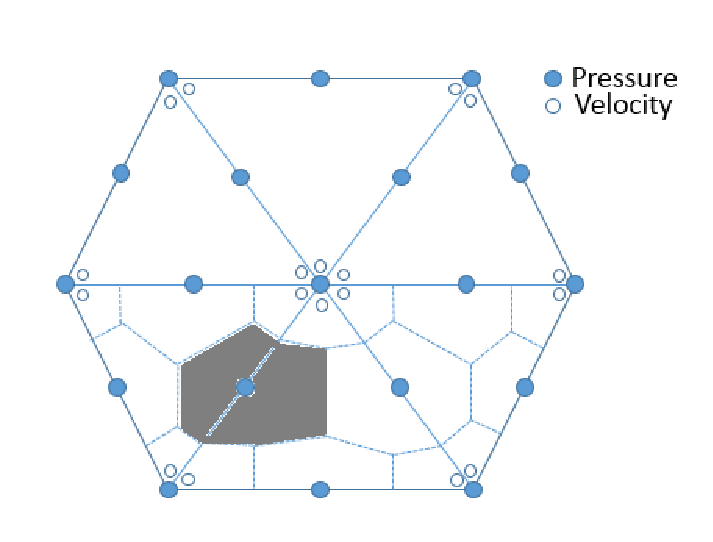
\includegraphics[width=.5\textwidth]{./Pics/P1DGP2.pdf}}
\caption{2D representation of \PN[1]{2} element pairs used in this work. Shaded areas denote control volumes across two contiguous elements. Blue and white circles represent pressure and velocity nodes, respectively.} 
\label{fig:fem_cv}
\end{figure}

\clearpage

%%%%
%%%%  FIGURE
%%%%
\begin{figure}[h]
\centering
\vbox{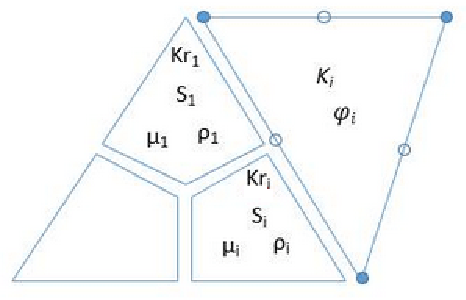
\includegraphics[width=.75\textwidth]{./Pics/element_n.pdf}}
\caption{This is a graphical representation of two different element types. Triangle {\it A} is a representation of the \PN[1]{2} element-pair, whereas triangle {\it B} represents the \PN[1]{1} element-pair. Porosity $\phi_{i}$, permeability {\bf K}$_{i}$, velocity and pressure are primarily represented in FE space whereas scalar fields (such as saturation, density, viscosity etc) are represented in CV space.}
\label{fig:fem_elem}
\end{figure}
\clearpage

%%%%
%%%%  FIGURE 
%%%%
\begin{figure}[h]
\centering
\vbox{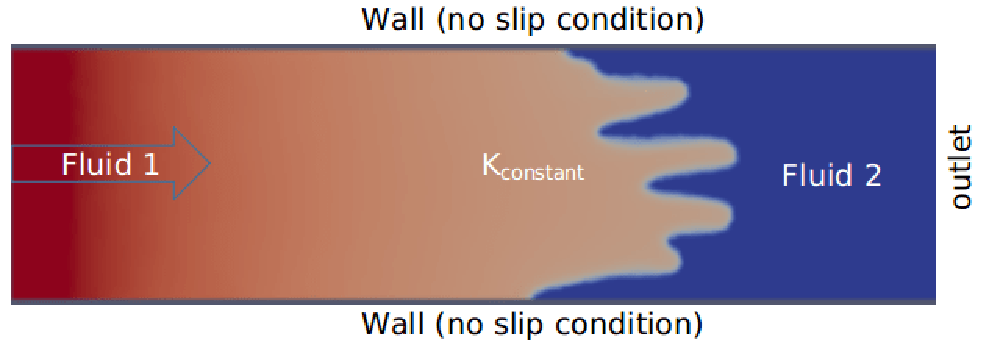
\includegraphics[width=0.75\textwidth]{./Pics/phase_vol_frac_uni_perm_1.pdf}}
\caption{Schematics of formation of flow instabilities during injection of a pure low viscosity fluid (red) into a domain saturated with a second fluid (dark blue). The ratio of viscosity between the two fluids is 5. In this case, the initially piston shape front collapses leading to the formation of several fingers.}
\label{fig:simple_case}
\end{figure}
\clearpage


%%%%
%%%%  FIGURE 
%%%%
\begin{figure}[ht] 
\vbox{
\hbox{\hspace{-0.3cm}
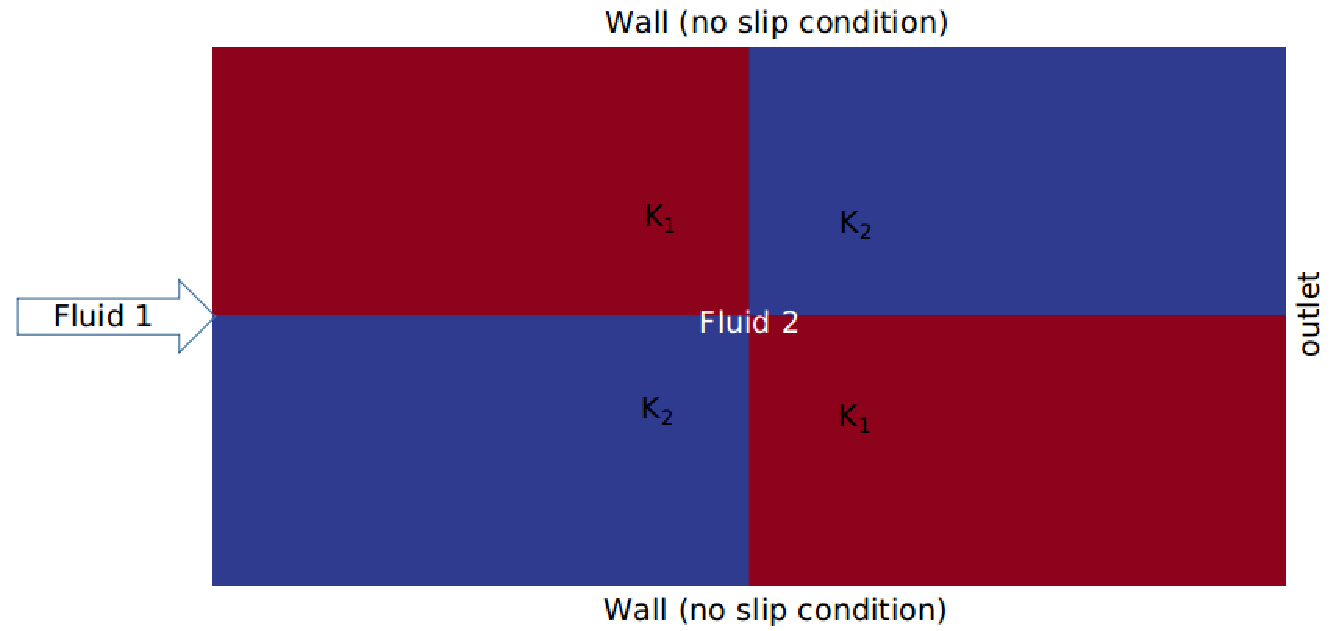
\includegraphics[width=.8\textwidth]{./Pics1/2b2_wi_fine/2b2_whole_in_fine_perm_1.pdf} 
}
\vspace{0.0cm}
\hbox{\hspace{3.5cm} (a) map of permeabilities ($\mathbf{K}$)
}
\vspace{0.25cm}
\hbox{\hspace{1.5cm}
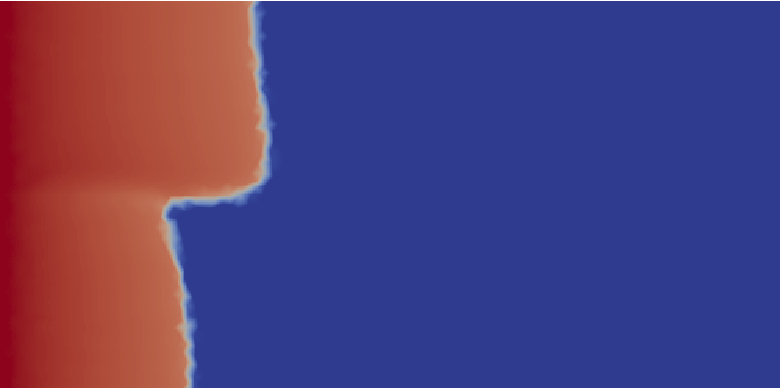
\includegraphics[width=.85\textwidth]{./Pics1/2b2_wi_fine/2b2_whole_in_fine_250_2.pdf}
}
\vspace{0.0cm}
\hbox{\hspace{4.5cm} (b) flow at t=250 
}
\vspace{0.25cm}
\hbox{\hspace{1.5cm}
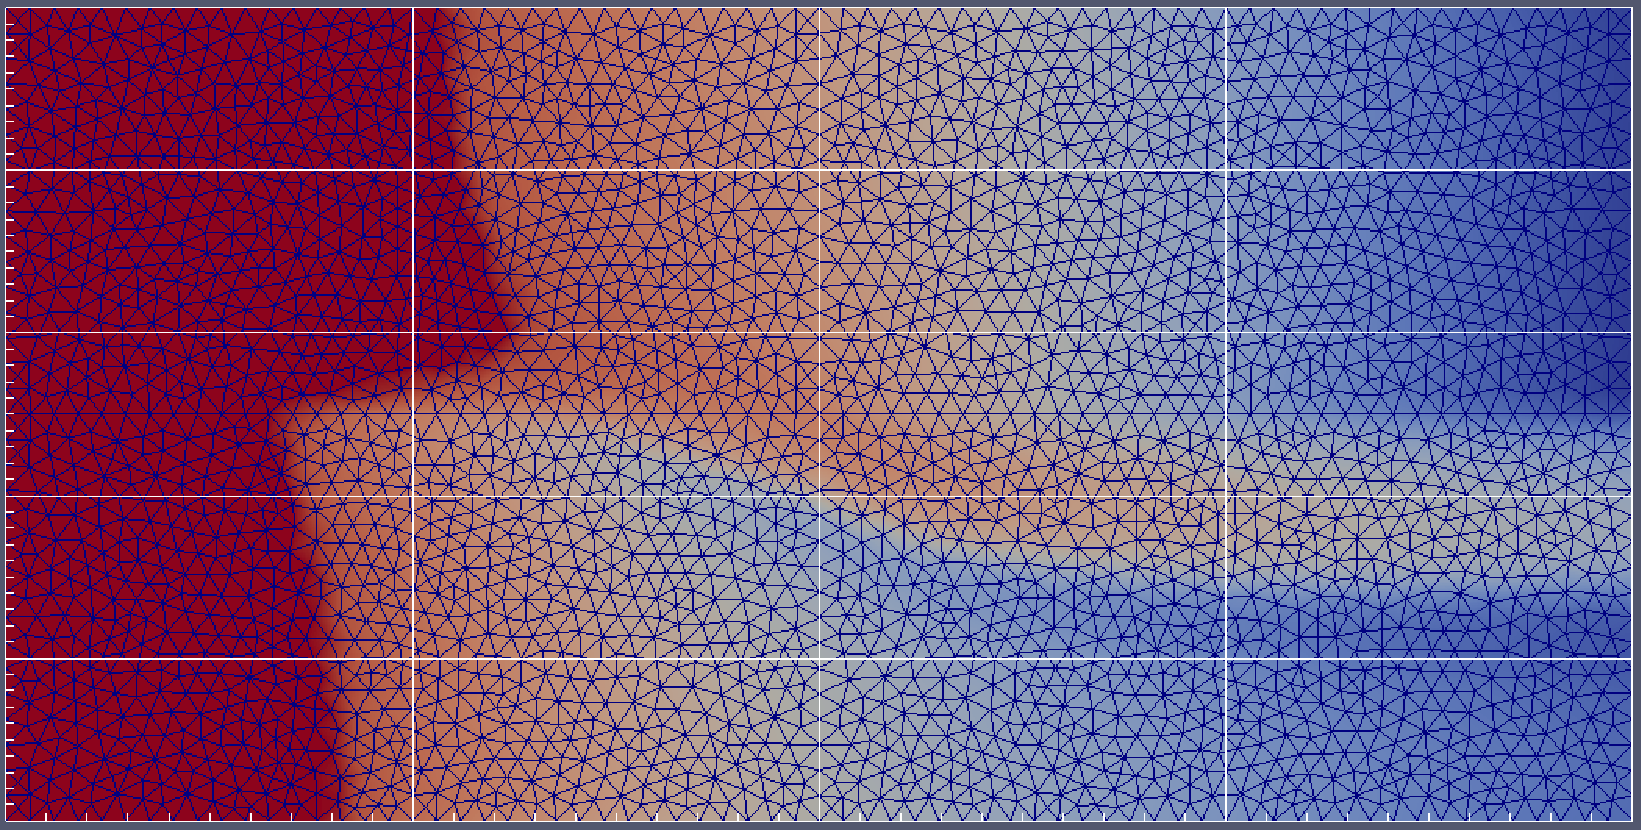
\includegraphics[width=.65\textwidth]{./Pics1/2b2_wi_fine/2b2_whole_in_fine_3000_2.pdf}
}
\vspace{0.0cm}
\hbox{\hspace{4.0cm} (c) flow at t=3000   
}}     
\caption{Model validation of fluid displacement in heterogeneous porous media ({\it VR}=1): (a) the domain is divided into four subdomains with prescribed synthetic permeability, $\mathbf{K}_{1}=1$ and $\mathbf{K}_{2}=2.5$; (b-c) snapshots of saturation (displacing fluid) field at t=$25$s and t=$300$ sec. The domain is discretised with $5960$ \PN[1]{2} elements. }
\label{fem_cv_represent_a}
\end{figure}
\clearpage



%%%%
%%%%  FIGURE
%%%%
\begin{landscape}
\begin{figure}[ht] 
\vbox{\vspace{-1cm}
\hbox{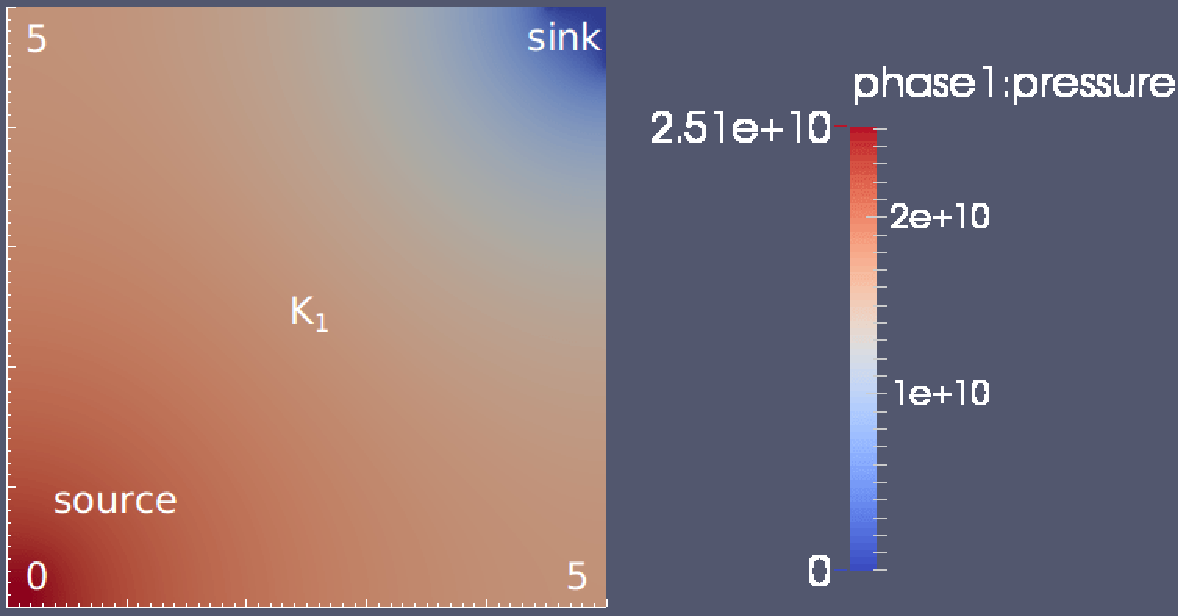
\includegraphics[width=.7\textwidth]{./Pics1/Saffman_homogeneous_MR3/saffman_homo_fixed_2.pdf}
      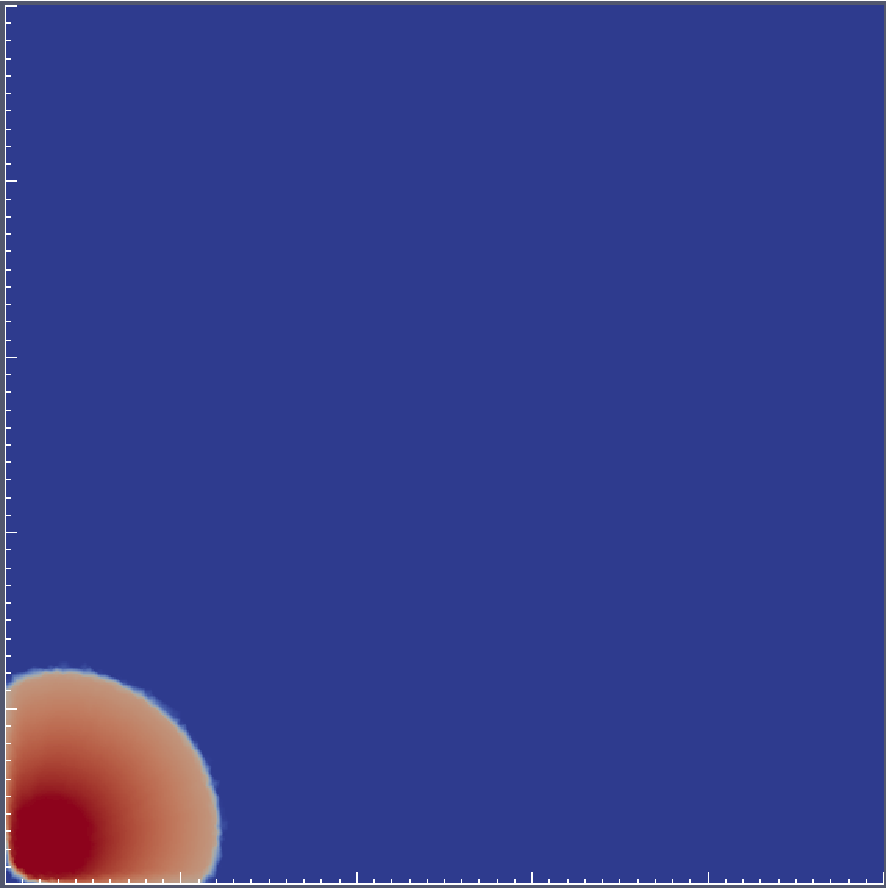
\includegraphics[width=.37\textwidth]{./Pics1/Saffman_homogeneous_MR3/saffman_homo_fixed_250.pdf}
      \includegraphics[width=.37\textwidth]{./Pics1/Saffman_homogeneous_MR3/saffman_homo_fixed_1000.pdf}}
\vspace{0.cm}
\hbox{\hspace{2.5cm} (a) pressure at t=0s \hspace{5.cm} (b) t=0.87s \hspace{2.75cm} (c) t=3.54s}
\vspace{0.5cm}
\hbox{
      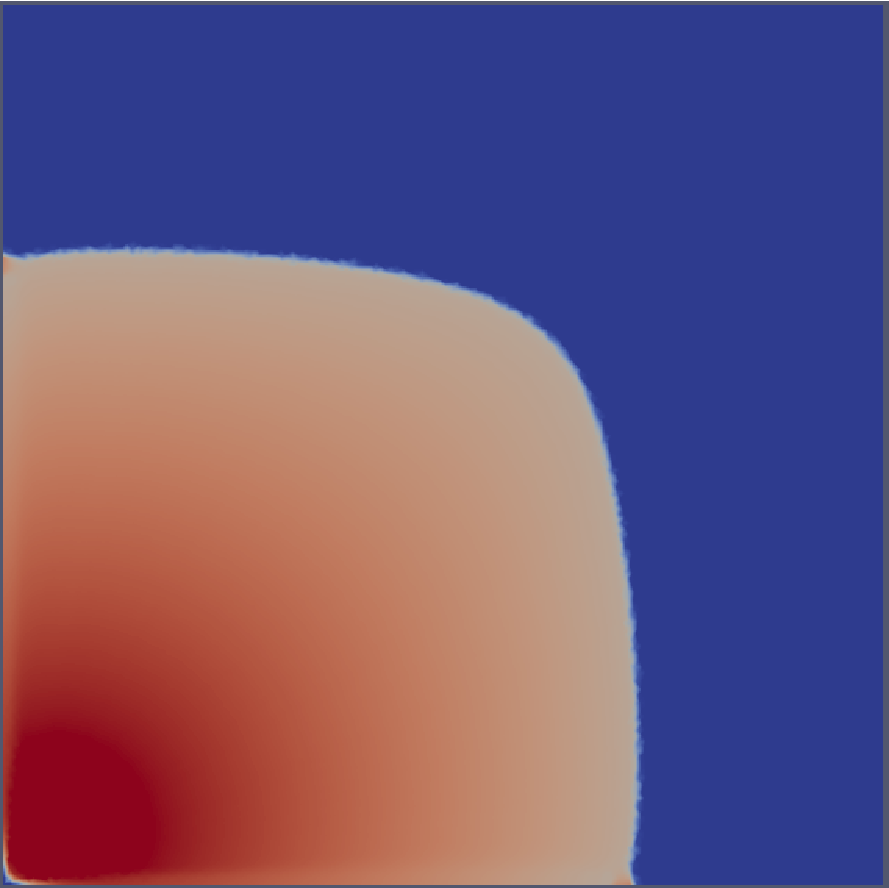
\includegraphics[width=.375\textwidth]{./Pics1/Saffman_homogeneous_MR3/saffman_homo_fixed_2500.pdf}
      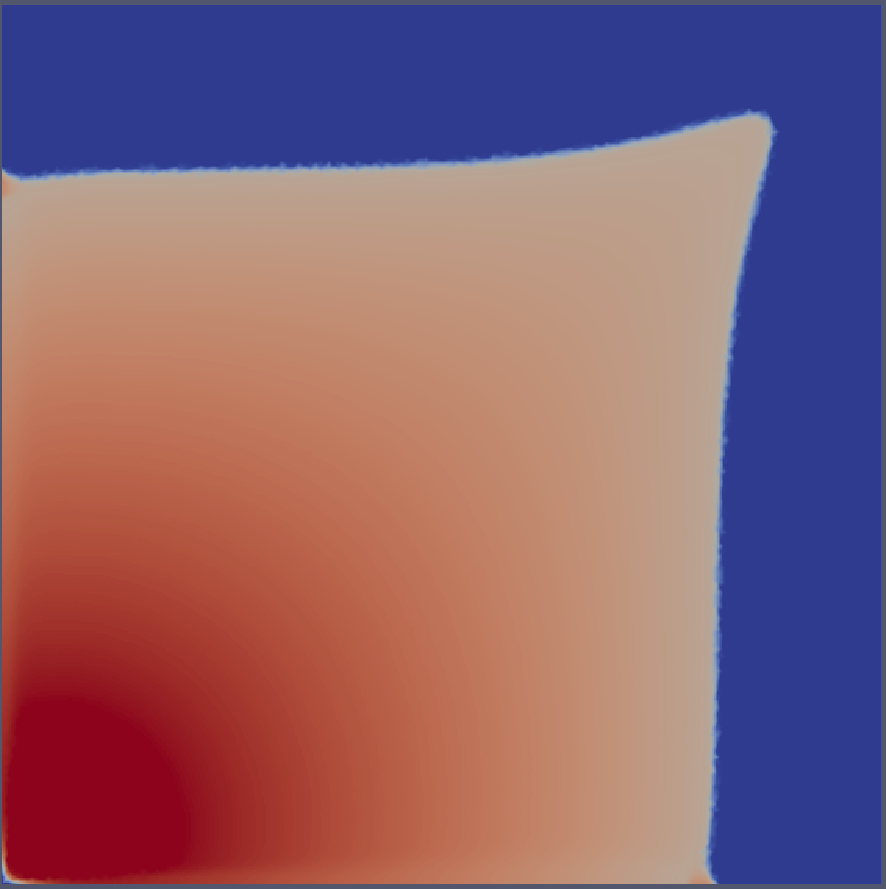
\includegraphics[width=.375\textwidth]{./Pics1/Saffman_homogeneous_MR3/saffman_homo_fixed_3500.pdf} 
      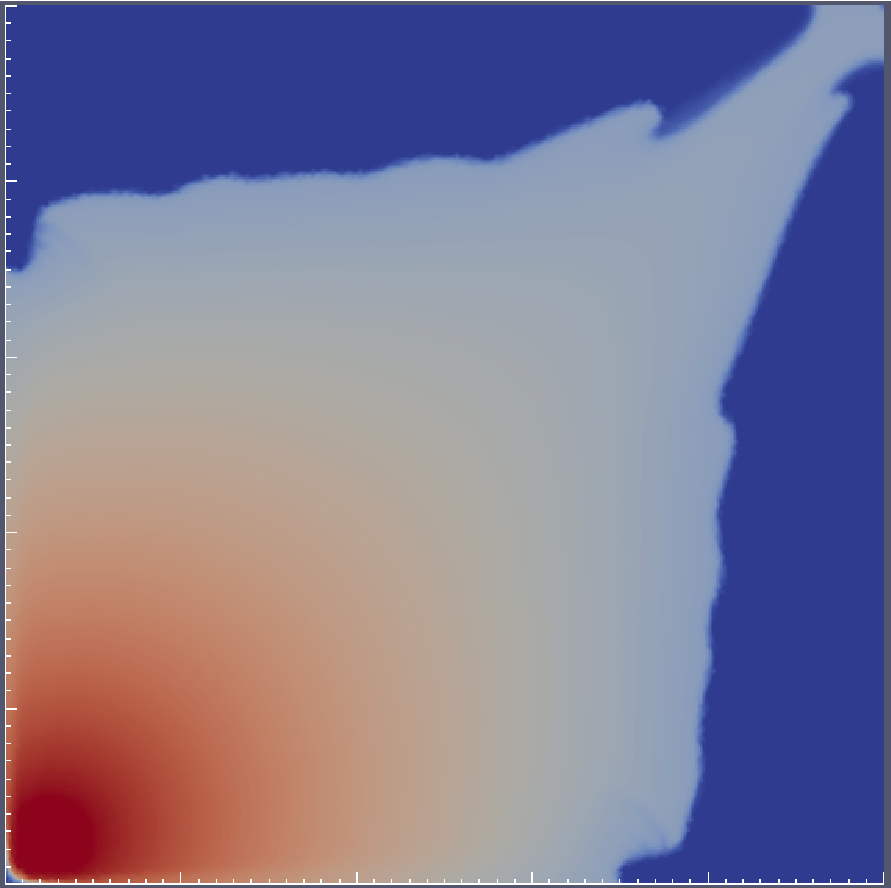
\includegraphics[width=.65\textwidth]{./Pics1/Saffman_homogeneous_MR3/saffman_homo_fixed_end.pdf}}
\vspace{0.cm}
\hbox{ \hspace{1.cm} (d) t=8.86s \hspace{3.0cm} (e) t=12.41s   \hspace{4.0cm} (f) t=17.95s}
\vspace{0.cm}
}   
\caption{Simulated flow in a Hele-Shaw cell ({\it VR}=3): (a) initial pressure profile $\left(\text{in g.cm}^{-1}\text{.s}^{-2}\right)$ with source and sink regions are explicitly shown along with dimensions (in cm); (b-f) snapshots of wetting phase saturation showing flow profile as the simulation evolves. The domain contains $47500$ \PN[1]{2} triangular elements.}
\label{fig:homoheleshaw_VN3}
\end{figure}
\end{landscape}
\clearpage



%%%%
%%%%  FIGURE
%%%%
\begin{landscape}
\begin{figure}[ht] 
\vbox{\vspace{-1cm}
\hbox{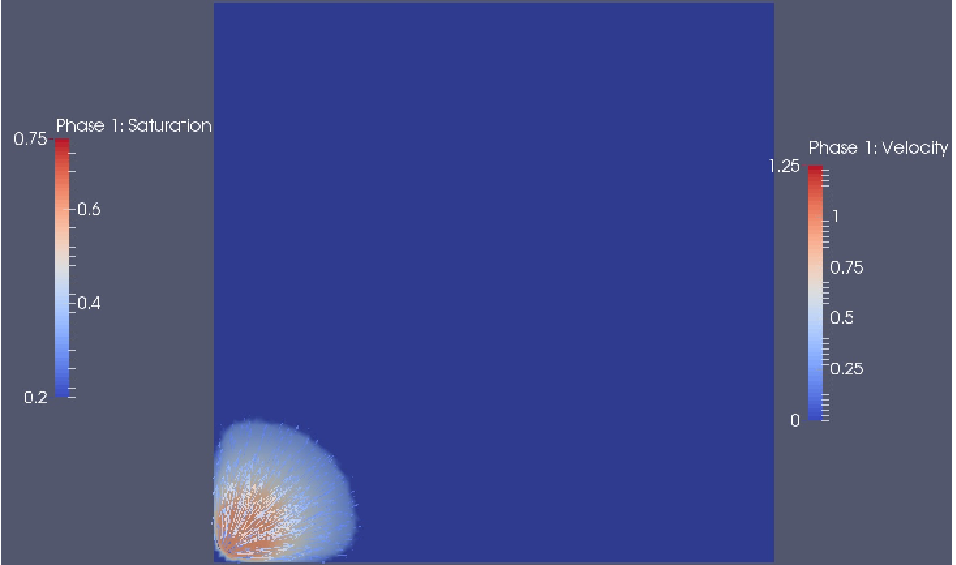
\includegraphics[width=.9\textwidth, height=0.5\textwidth]{./Pics1/Saffman_homogeneous_VR10/ST_Homog_VR10_D201c.pdf}
\hspace{0.5cm}      
      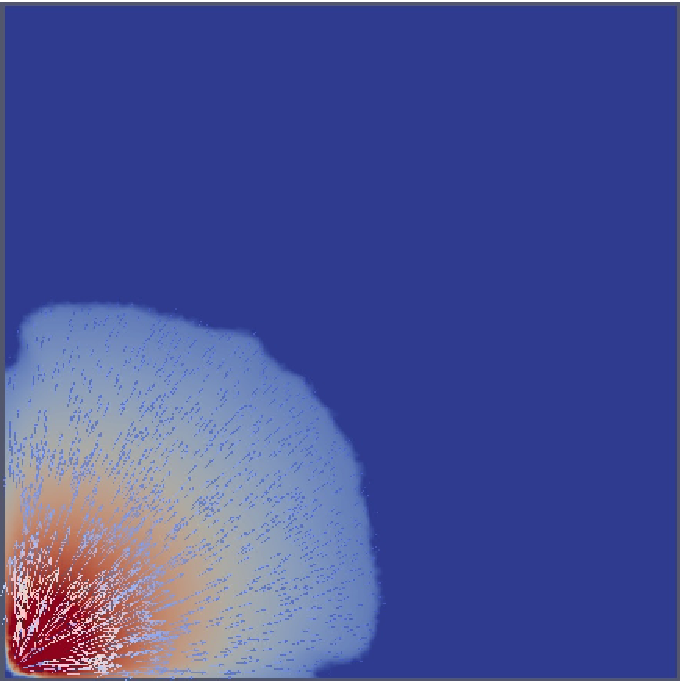
\includegraphics[width=.5\textwidth]{./Pics1/Saffman_homogeneous_VR10/ST_Homog_VR10_D1001c.pdf}}
\vspace{0.cm}
\hbox{\hspace{5.cm} (a) t=0.66s \hspace{8.cm} (b) t=3.43s }
\vspace{0.5cm}
\hbox{
      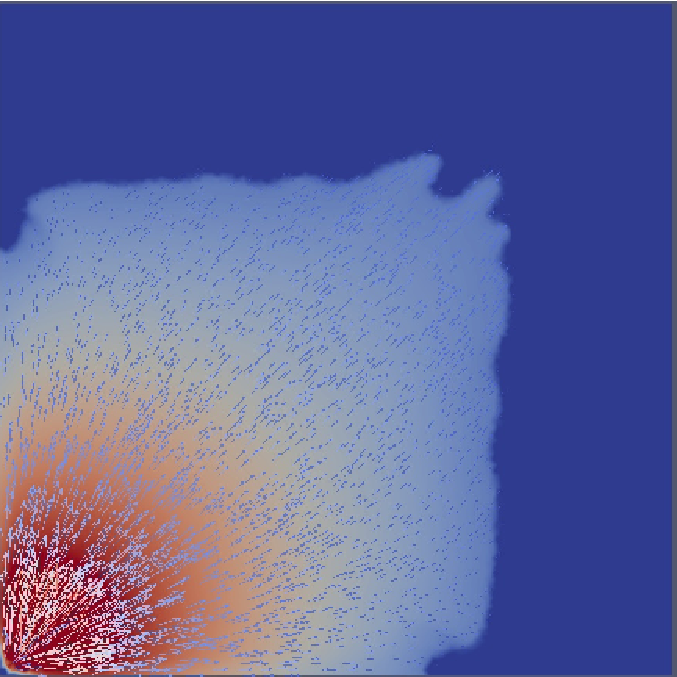
\includegraphics[width=.5\textwidth]{./Pics1/Saffman_homogeneous_VR10/ST_Homog_VR10_D2001c}
      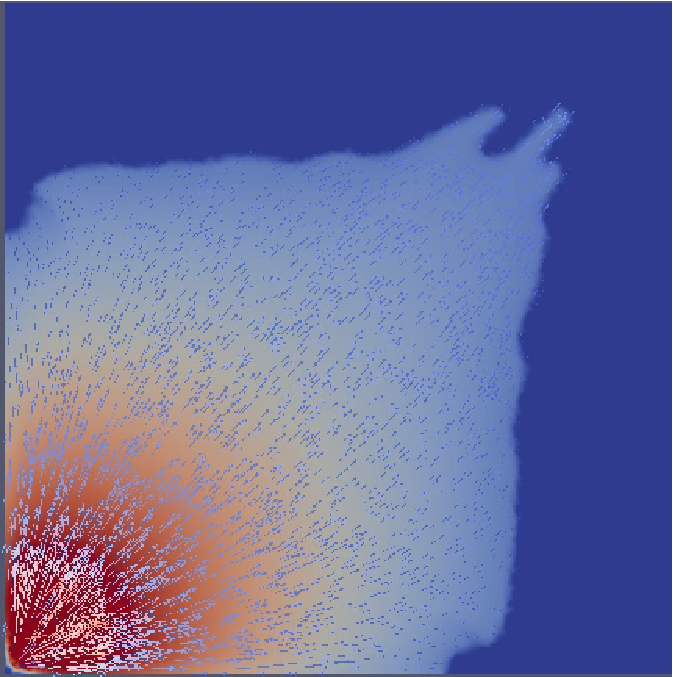
\includegraphics[width=.5\textwidth]{./Pics1/Saffman_homogeneous_VR10/ST_Homog_VR10_D2201c}
      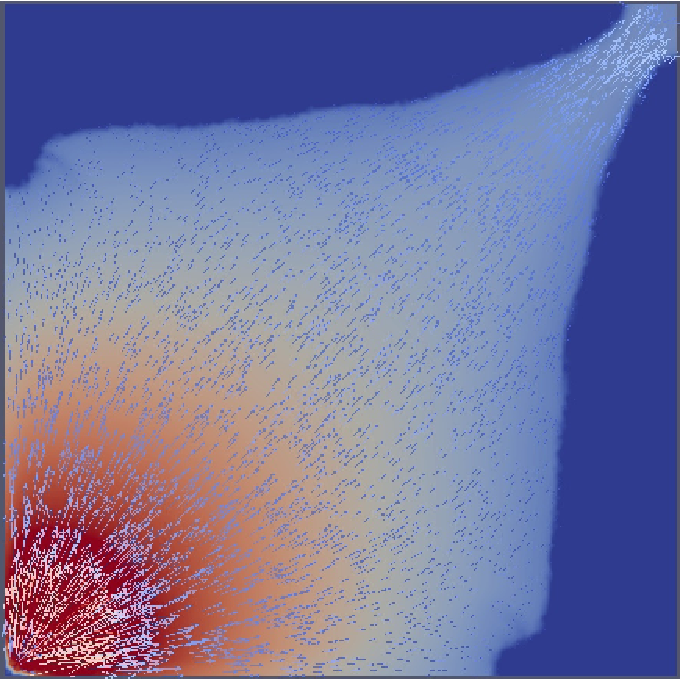
\includegraphics[width=.5\textwidth]{./Pics1/Saffman_homogeneous_VR10/ST_Homog_VR10_D3001c}}
\vspace{0.cm}
\hbox{ \hspace{2.cm} (c) t=6.92s \hspace{4.5cm} (d) t=7.61s \hspace{4.5cm} (e)t=10.00s}
\vspace{0.cm}
}   
\caption{Simulated flow in a Hele-Shaw cell ({\it VR}=10): snapshots of overlapped wetting phase saturation and velocity vectors showing flow profile as the simulation evolves. The domain contains $26313$ \PN[1]{2} triangular elements.}
\label{fig:homoheleshaw_VN10}
\end{figure}
\end{landscape}
\clearpage

%%%%
%%%%  FIGURE
%%%%
\begin{landscape}
\begin{figure}[ht] 
\vbox{\vspace{-1cm}
\hbox{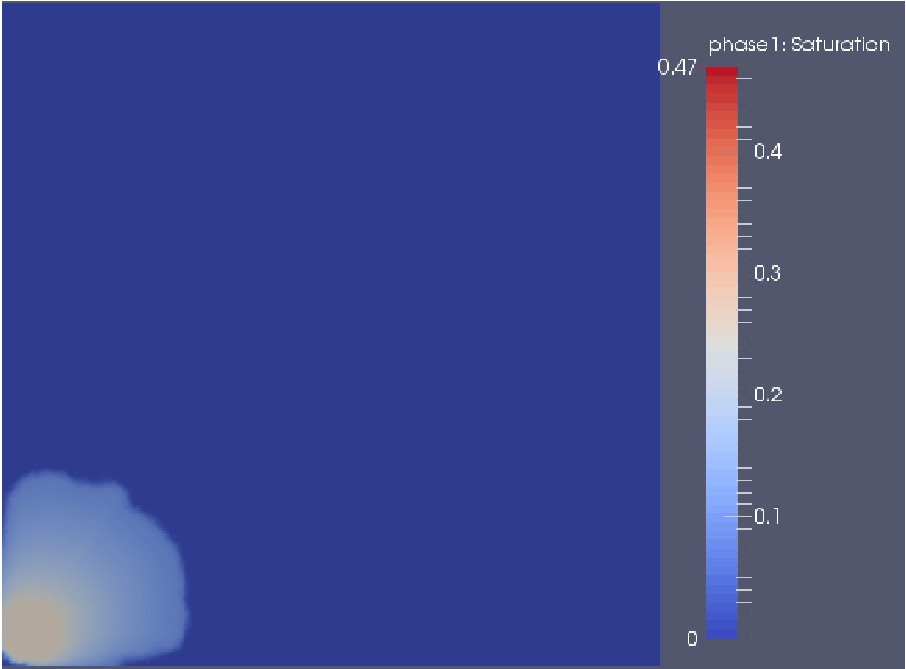
\includegraphics[width=.9\textwidth, height=0.5\textwidth]{./Pics1/Saffman_homogeneous_VR150/ST_Homog_VR150_D300b}
\hspace{0.5cm}      
      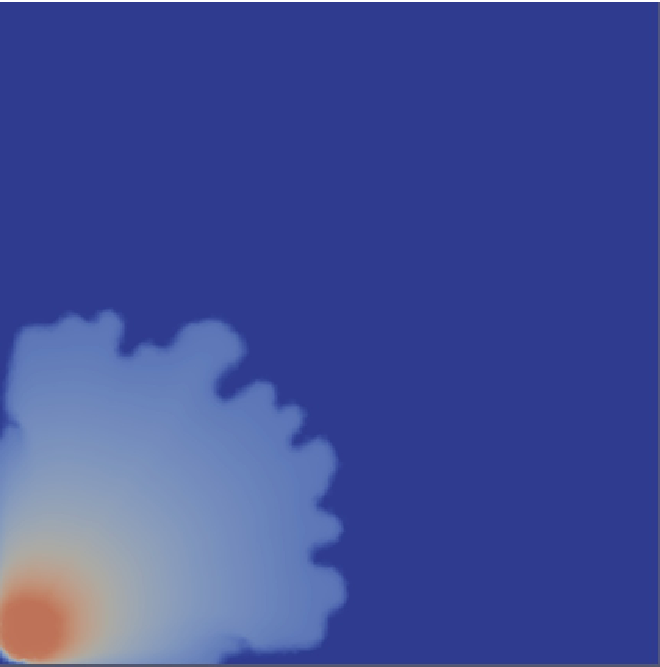
\includegraphics[width=.5\textwidth]{./Pics1/Saffman_homogeneous_VR150/ST_Homog_VR150_D1600b}}
\vspace{0.cm}
\hbox{\hspace{5.cm} (a) t=0.27s \hspace{8.cm} (b) t=0.94s }
\vspace{0.5cm}
\hbox{
      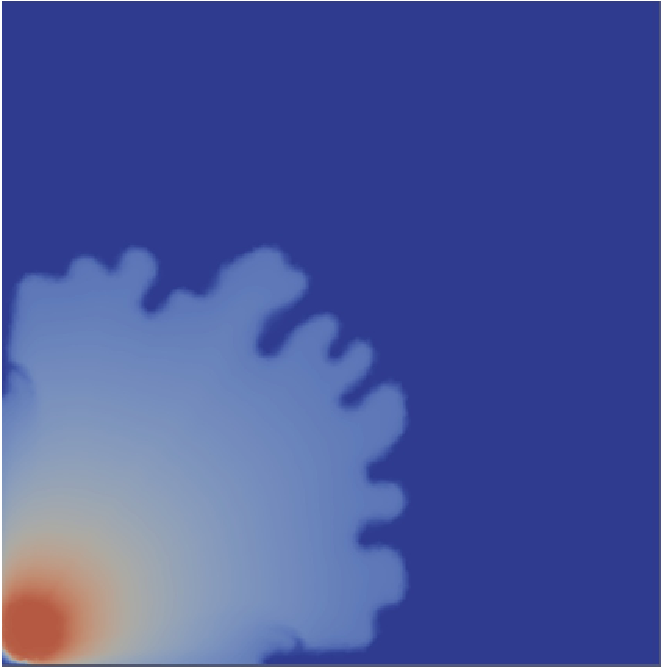
\includegraphics[width=.5\textwidth]{./Pics1/Saffman_homogeneous_VR150/ST_Homog_VR150_D2700b}
      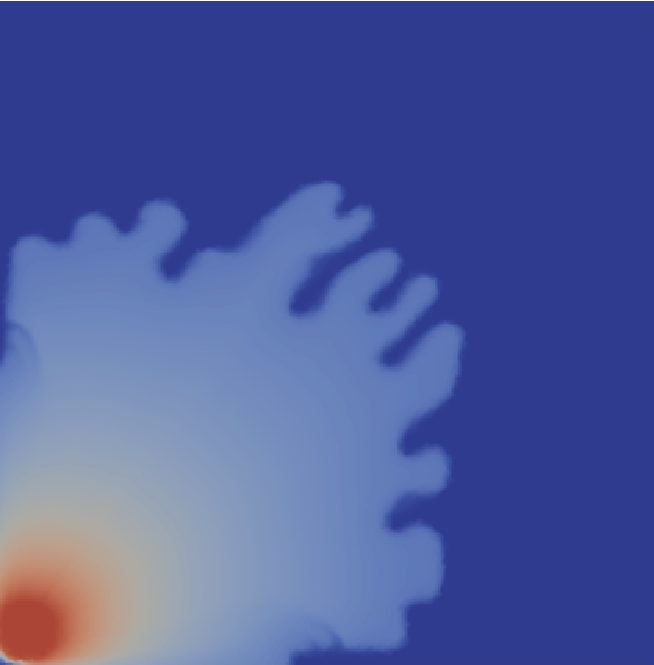
\includegraphics[width=.5\textwidth]{./Pics1/Saffman_homogeneous_VR150/ST_Homog_VR150_D4000b}
      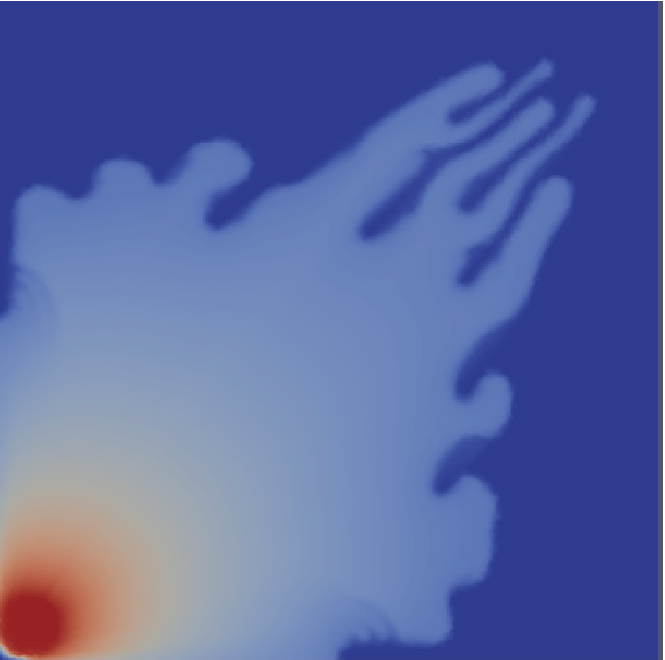
\includegraphics[width=.5\textwidth]{./Pics1/Saffman_homogeneous_VR150/ST_Homog_VR150_D7000b}}
\vspace{0.cm}
\hbox{ \hspace{2.cm} (c) t=1.32s \hspace{4.5cm} (d) t=1.70s \hspace{4.5cm} (e)t=2.31s}
\vspace{0.cm}
}   
\caption{Simulated flow in a Hele-Shaw cell ({\it VR}=150): snapshots of wetting phase saturation showing flow profile as the simulation evolves. The domain contains $26313$ \PN[1]{2} triangular elements.}
\label{fig:homoheleshaw_VN10}
\end{figure}
\end{landscape}
\clearpage


%%%%
%%%%  FIGURE
%%%%
\begin{landscape}
\begin{figure}[ht] 
\hbox{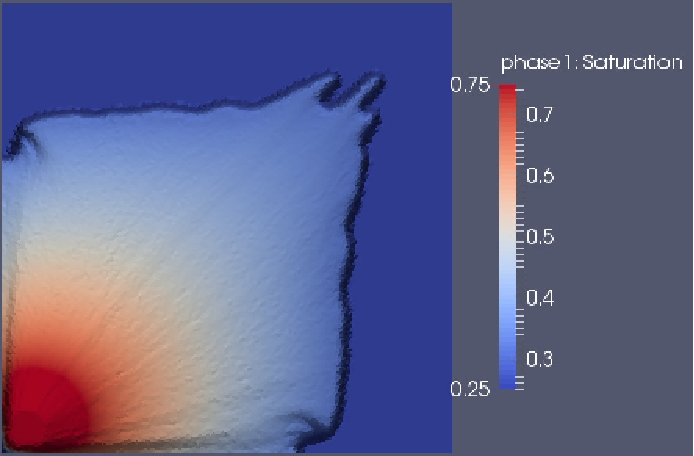
\includegraphics[width=.5\textwidth]{./Pics1/Saffman_homogeneous_VR10/ST_Homog_VR10_D2201_bbd}
       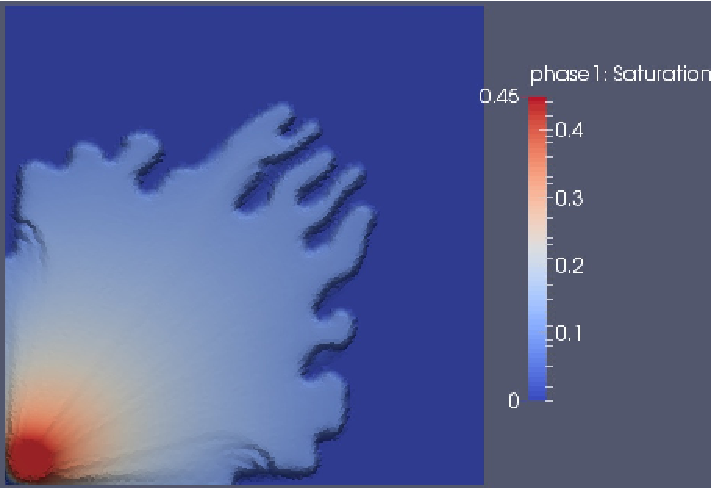
\includegraphics[width=.49\textwidth]{./Pics1/Saffman_homogeneous_VR150/ST_Homog_VR150_D5003_k2b}}
\caption{Simulated flow in Hele-Shaw cells performed with viscosity ratios of 10 (left, t=7.61s) and 150 (t=1.94s). Width of largest fingers are approximetely 0.70 and 0.90cm, which are in good agreement with values obtained from \citet{guan_2003}'s analytic solution. Domains of both simulations contain $26313$ \PN[1]{2} triangular elements.\red{(More pics to be added!!)}}
\label{fig:homoheleshaw_VN10_VN150}
\end{figure}
\end{landscape}



\begin{comment}

%%%%
%%%%  FIGURE
%%%%
\begin{landscape}
\begin{figure}[ht] 
\vbox{\vspace{-1cm}
\hbox{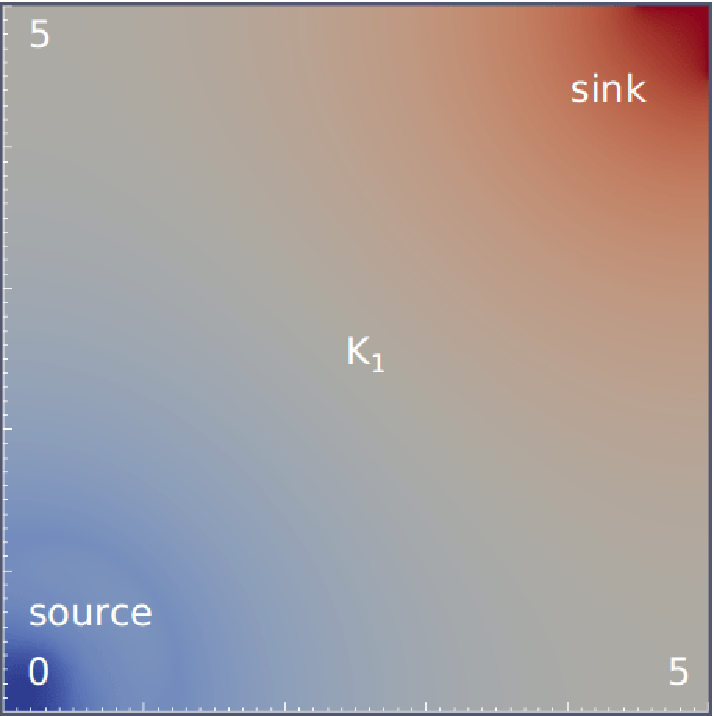
\includegraphics[width=.5\textwidth]{./Pics1/Saffman_homogeneous/saffman_homo_fixed_1.pdf}
      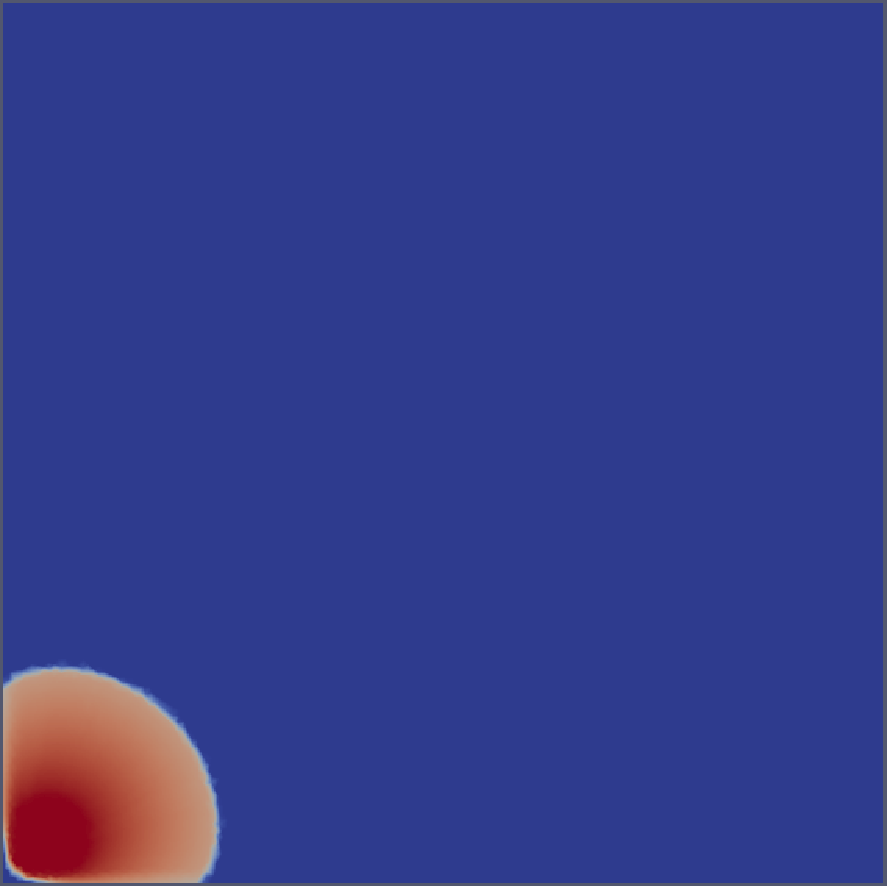
\includegraphics[width=.5\textwidth]{./Pics1/Saffman_homogeneous/saffman_homo_fixed_250_1.pdf}
      \includegraphics[width=.5\textwidth]{./Pics1/Saffman_homogeneous/saffman_homo_fixed_1000.pdf}}
\vspace{0.cm}
\hbox{\hspace{1.0cm} (a) pressure at t=0 \hspace{3.cm} (b) t=250\red{(???)} \hspace{3.0cm} (c) t=1000\red{(???)}}
\vspace{0.5cm}
\hbox{
      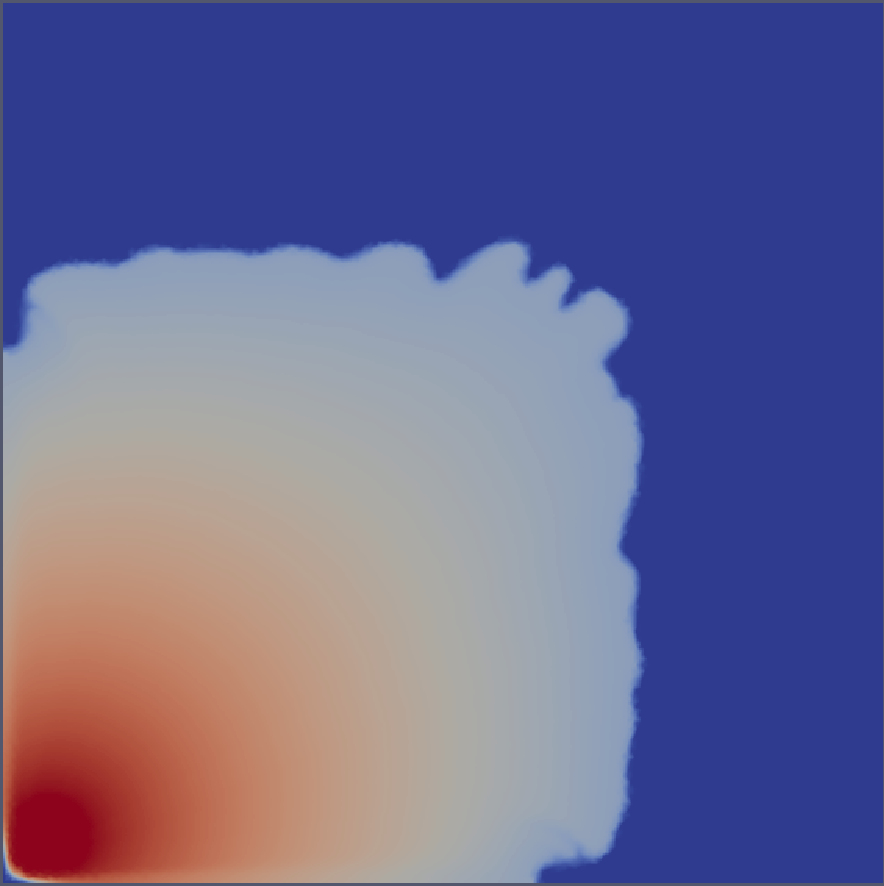
\includegraphics[width=.5\textwidth]{./Pics1/Saffman_homogeneous/saffman_homo_fixed_6000.pdf}
      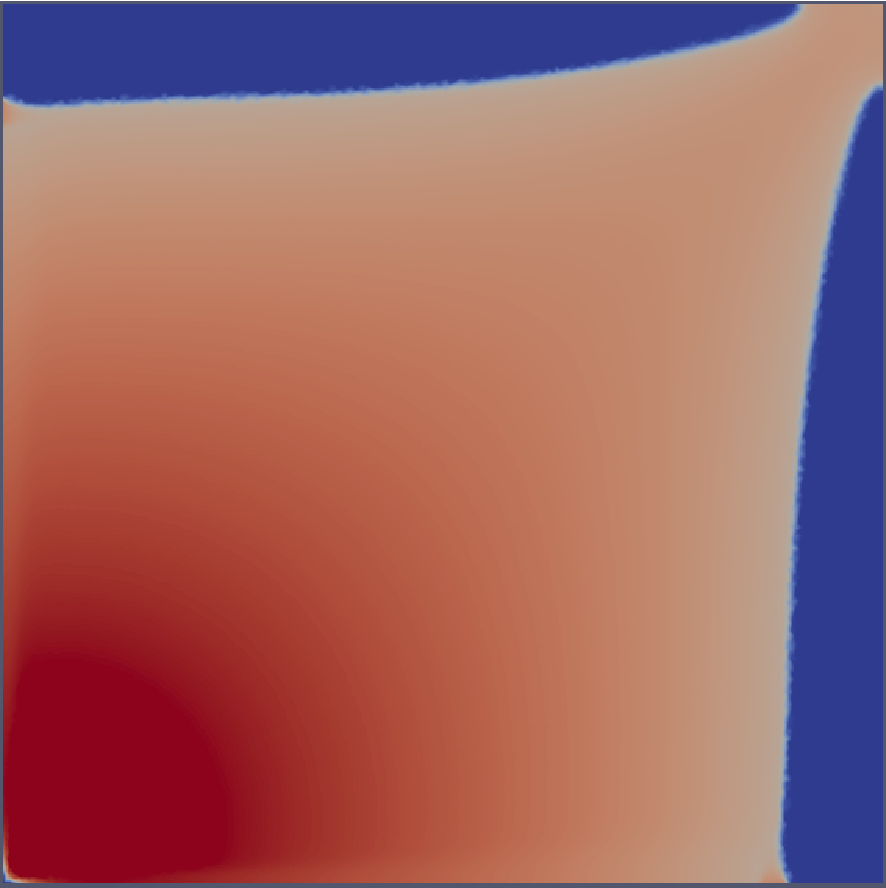
\includegraphics[width=.5\textwidth]{./Pics1/Saffman_homogeneous/saffman_homo_fixed_end_1.pdf}}
\vspace{0.cm}
\hbox{ \hspace{2.cm} (d) t=6000\red{(???)} \hspace{3.cm} (e) t=XXX\red{(???)}}
\vspace{0.cm}
}   
\caption{Simulated flow in a Hele-Shaw cell ({\it VR}=10): (a) pressure profile $\left(\text{in g.cm}^{-1}\text{.s}^{-2}\right)$ with source and sink regions explicitly shown along with dimensions (in cm); (b-e) snapshots of wetting phase saturation showing flow profile as the simulation evolves. The domain contains $47000$ \PN[1]{2} triangular elements. The pressure and saturation range of values are the same like the  case in fig.\ref{fig:homoheleshaw_VN3}.}
\label{fig:homoheleshaw_VN10}
\end{figure}
\end{landscape}
\clearpage
\end{comment}


%%%
%%% FIGURE XXXXXX
%%%
\begin{landscape}
  \begin{figure}[ht]
  \vbox{\vspace{-1cm}
      \hbox{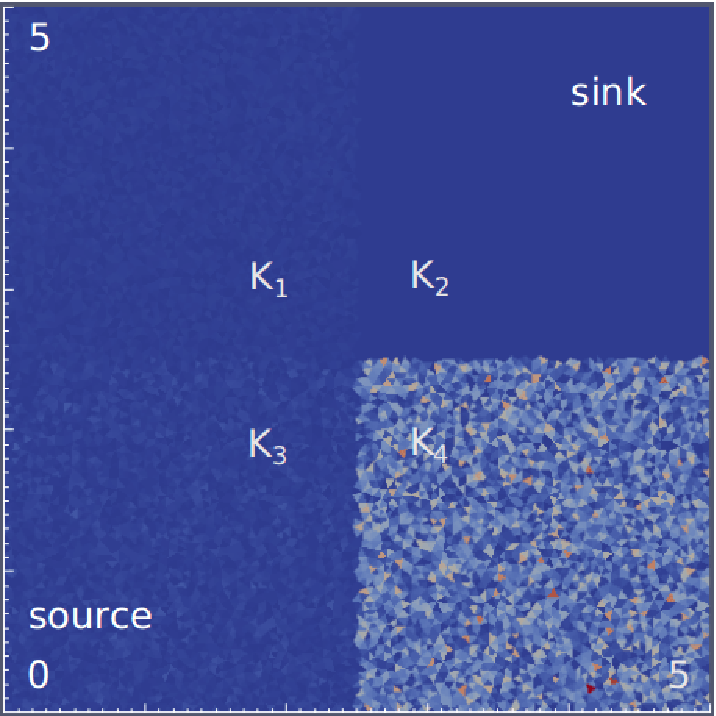
\includegraphics[width=.5\textwidth]{./Pics1/Saffman_heterogeneous/saffman_heter_fixed_1.pdf}
            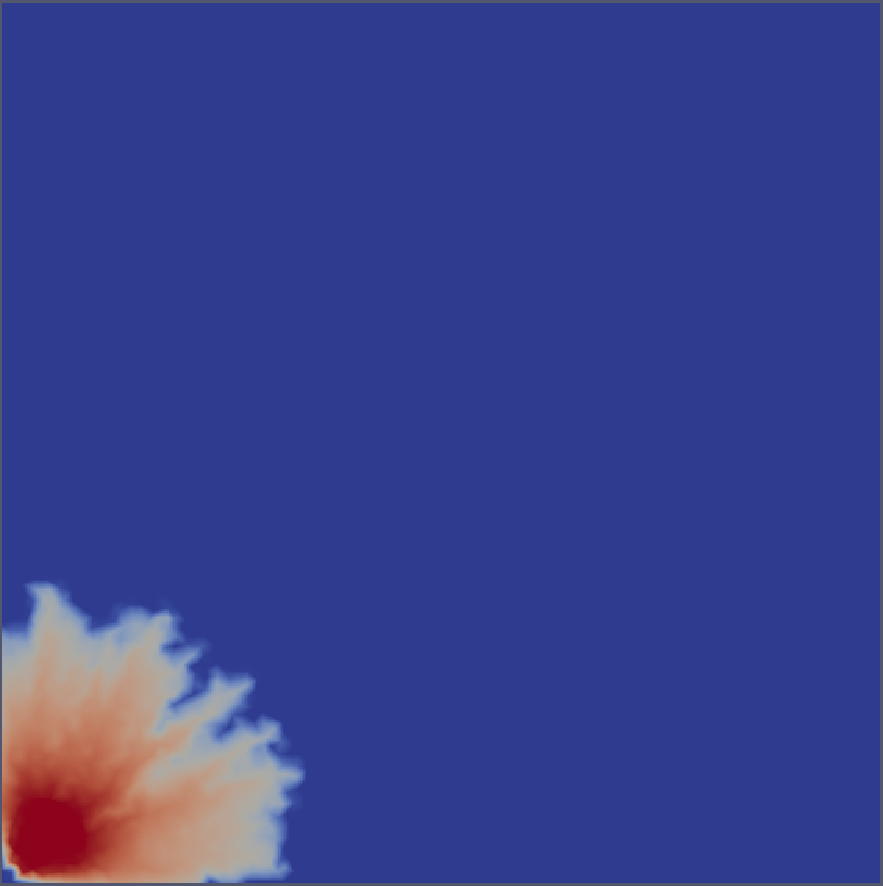
\includegraphics[width=.5\textwidth]{./Pics1/Saffman_heterogeneous/saffman_heter_fixed_500.pdf} 
            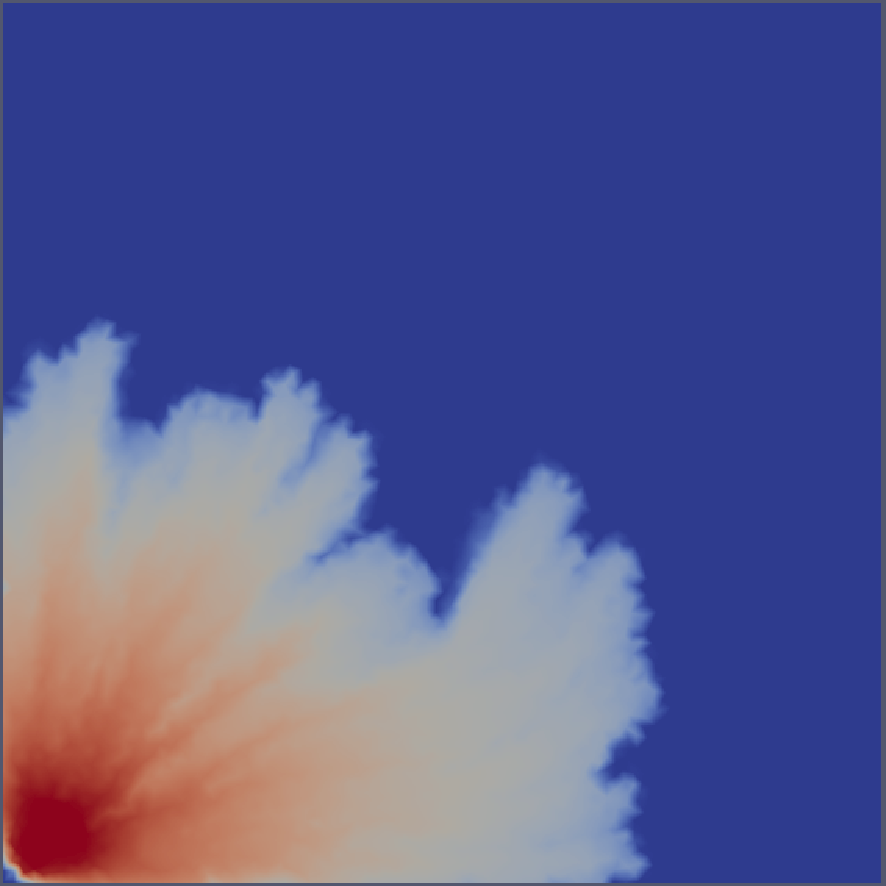
\includegraphics[width=.5\textwidth]{./Pics1/Saffman_heterogeneous/saffman_heter_fixed_2000.pdf} }
      \hbox{\hspace{1.0cm} (a) permeability map \hspace{3.cm} (b) t=0.75s \hspace{4.0cm} (c) t=8s}
      \vspace{0.5cm}
      \hbox{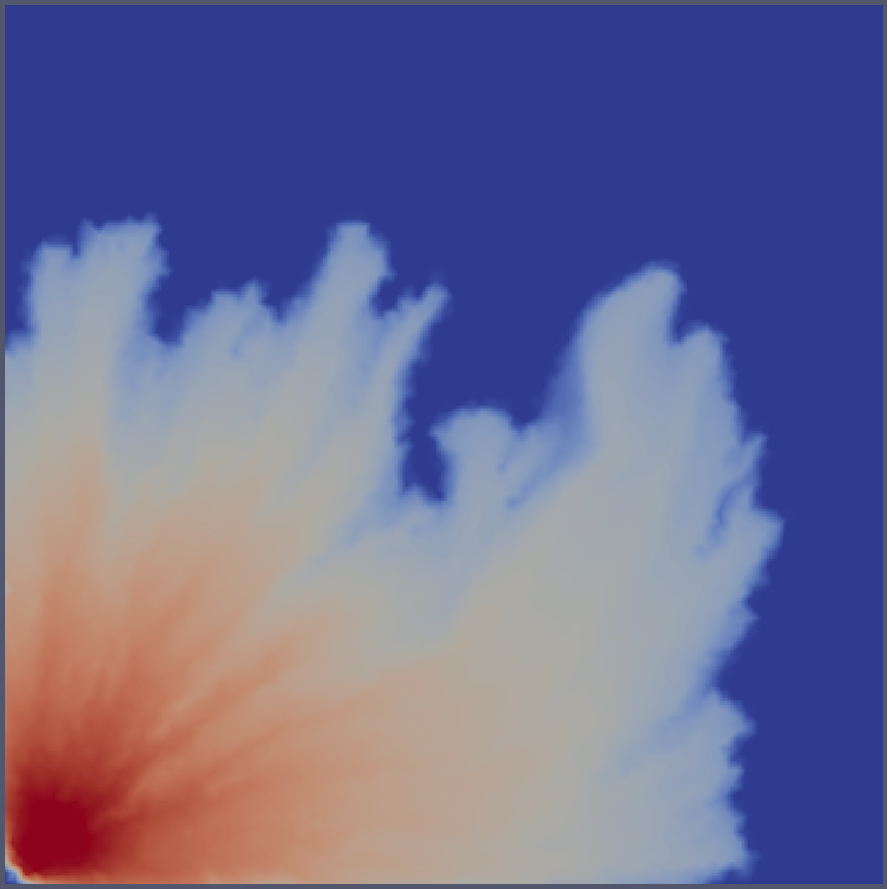
\includegraphics[width=.5\textwidth]{./Pics1/Saffman_heterogeneous/saffman_heter_fixed_3000.pdf}
            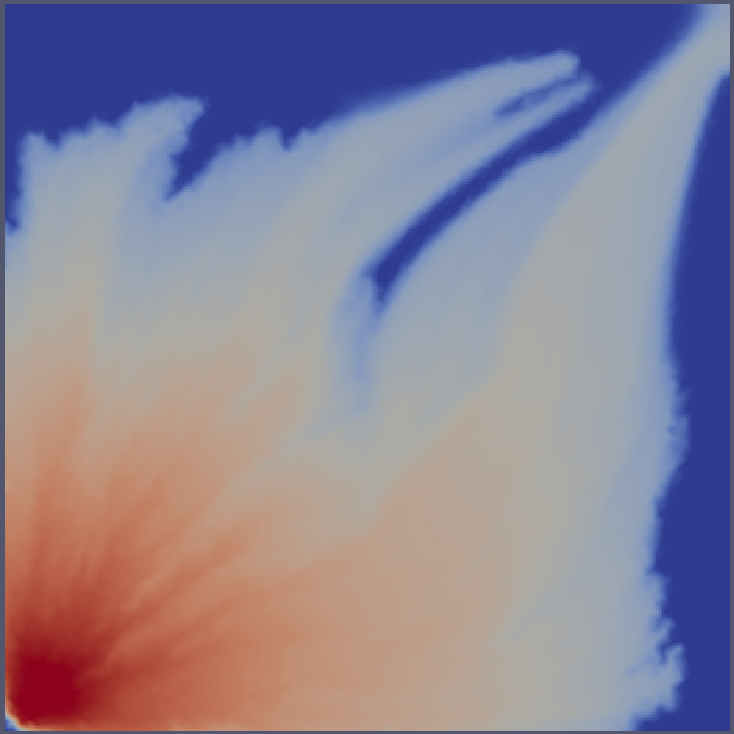
\includegraphics[width=.5\textwidth]{./Pics1/Saffman_heterogeneous/saffman_heter_fixed_6000.pdf}
            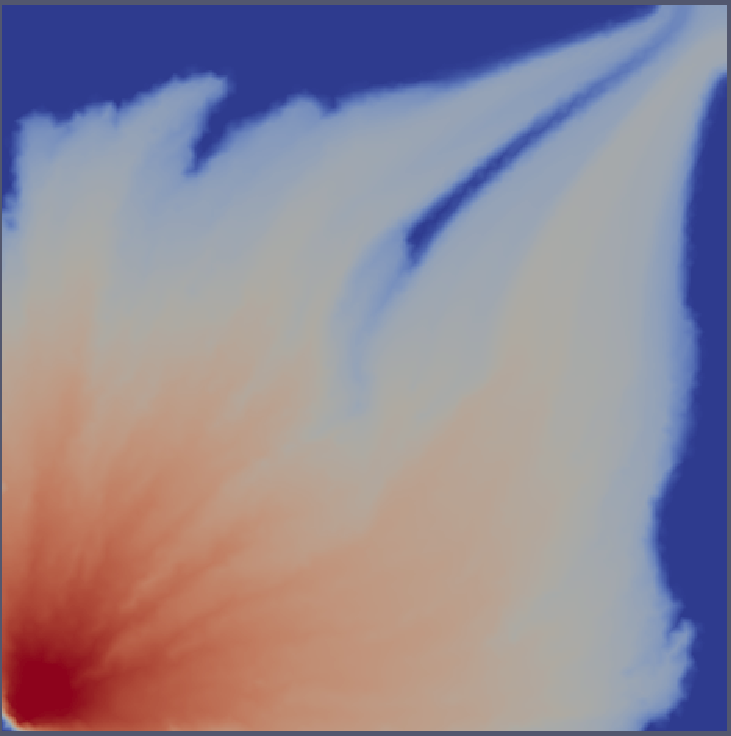
\includegraphics[width=.5\textwidth]{./Pics1/Saffman_heterogeneous/saffman_heter_fixed_24000.pdf} }
      \hbox{\hspace{2.5cm} (d) t=18s \hspace{5.cm} (e) t= \hspace{3.0cm} (f) t=24000 }}
\caption{Simulated flow in a modified Hele-Shaw cell with {\it VR}=10: (a) permeability distribution $\left(\text{10}^{-10}\le\mathbf{K}_{1}\le\text{5}\times\text{10}^{-10}\right.$, {\bf K}$_{2}$=10$^{-10}$, 10$^{-11}\le\mathbf{K}_{3}\le$ 5$\times$10$^{-10}$ and 10$^{-12}\le\mathbf{K}_{4}\le$ 5$\times$10$\left.^{-10}\text{ cm}^{2}\right)$; (b-f) snapshots of saturation profile during \red{XX} seconds of simulation. The domain contains \red{XX} \PN[1]{2} element-pairs.}
\label{fig:HeleShawHeter_VR10}
\end{figure}
\end{landscape}
\clearpage



%%%%
%%%%  FIGURE
%%%%
\begin{landscape}
\begin{figure}[ht] 
\vbox{
\hbox{\hspace{4.0cm}
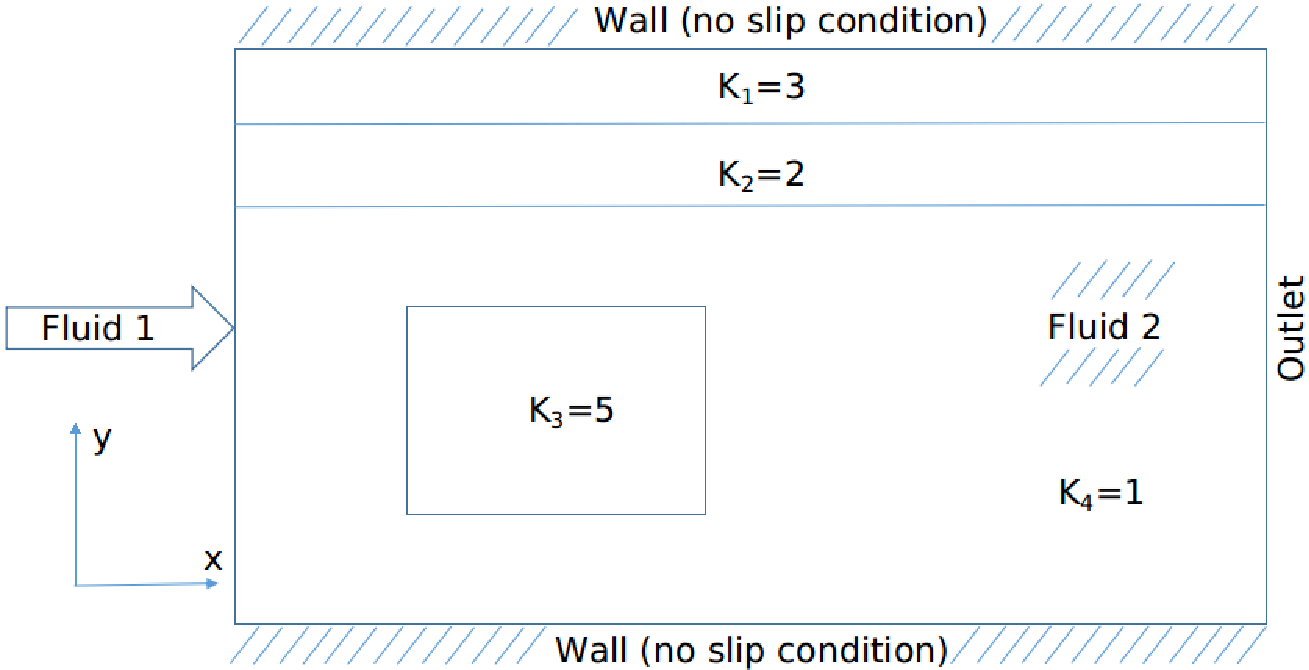
\includegraphics[width=.75\textwidth]{./Pics/map_of_boundaries.pdf} 
}
\vspace{0.0cm}
\hbox{\hspace{6.5cm} (a) map of permeabilties K   
}
\vspace{0.25cm}
\hbox{\hspace{4.0cm}
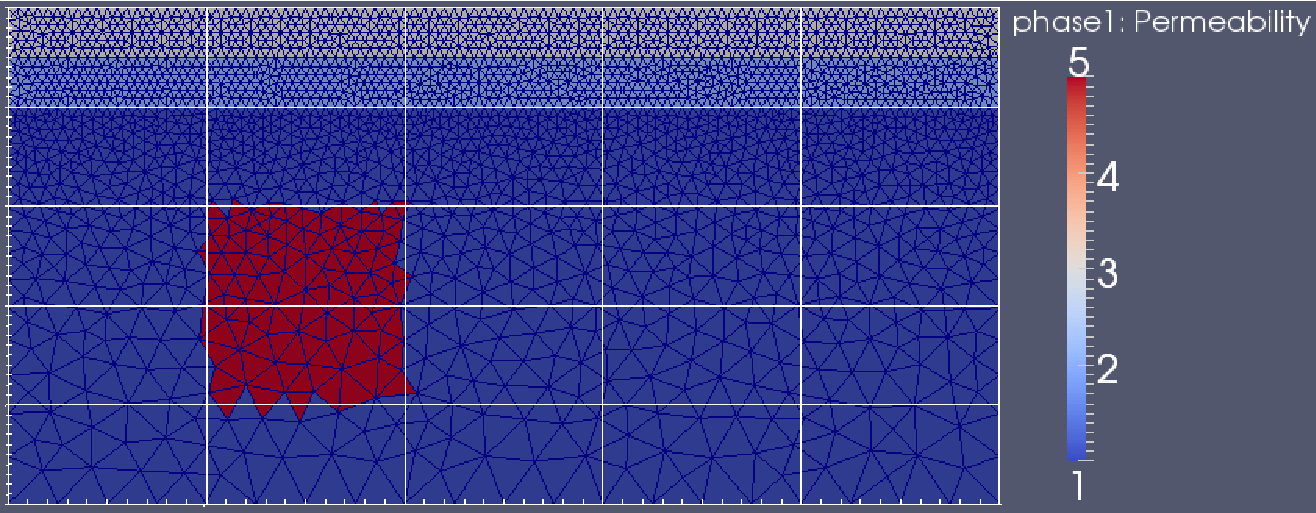
\includegraphics[width=.9\textwidth]{./Pics/map_of_boundaries_1.pdf}
}
\vspace{0.0cm}
\hbox{\hspace{9cm} (b)      
}
}     
\caption{Figure (a) describes the initial and boundary conditions as these are applied in this set of simulations. Below (b) there is a comparison between the unstructured and fixed mesh and the unstructured and adaptive mesh. During the implementation of fixed mesh initially there $4606$ elements while for the adaptive mesh there are $606$ while the majority of them is on the interface between between the two fluids. }
\label{fig:testcase_heter_domain}
\end{figure}
\end{landscape}
\clearpage



%%%%
%%%%  FIGURE
%%%%
\begin{landscape}
\begin{figure}[ht] 
\vbox{
\hbox{\hspace{3.5cm}
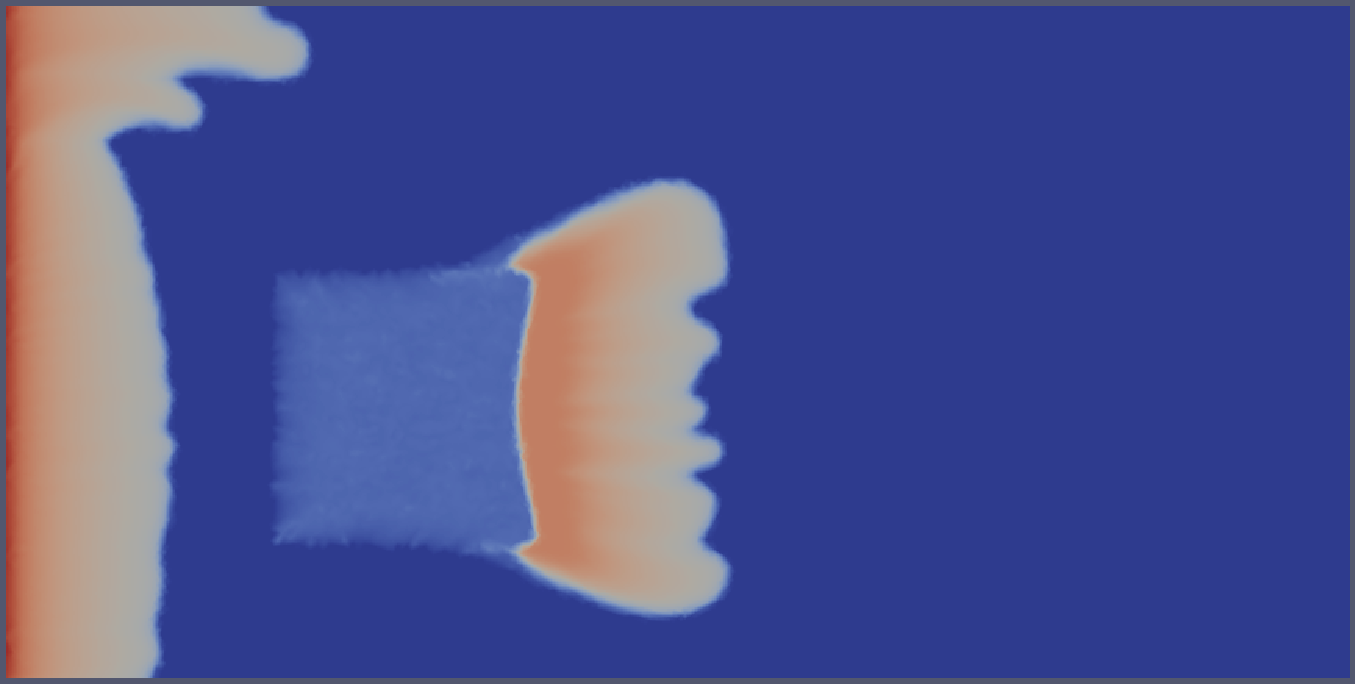
\includegraphics[width=.65\textwidth]{./Pics1/mr10_5regions_fixed/5regions_fixed_250.pdf} 
}
\vspace{0.0cm}
\hbox{\hspace{6.5cm} (a) flow at t=250 (fixed mesh)  
}
\vspace{0.25cm}
\hbox{\hspace{3.5cm}
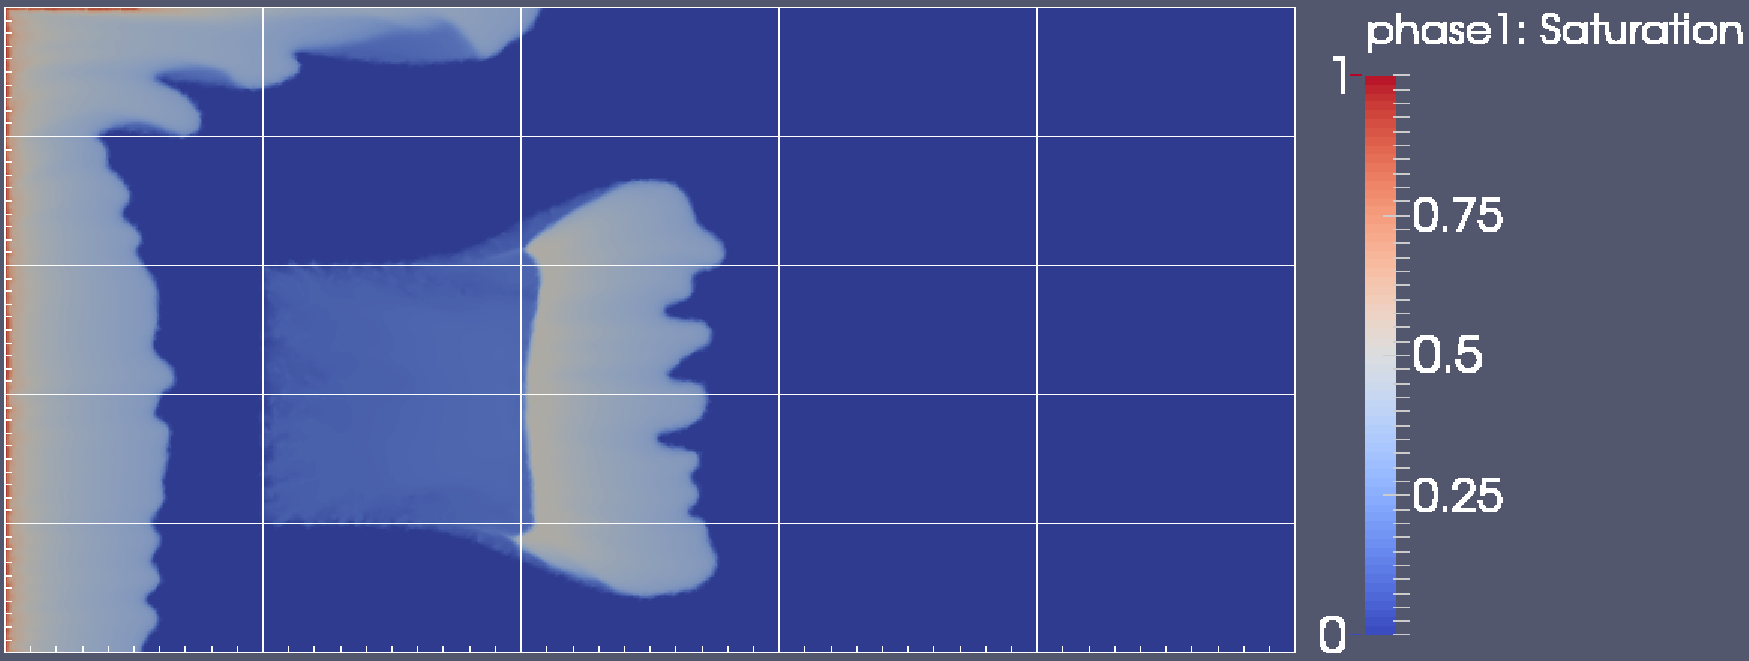
\includegraphics[width=.9\textwidth]{./Pics1/mr10_5regions_adapt/5regions_adapt_250_1.pdf}
}
\vspace{0.0cm}
\hbox{\hspace{6.5cm} (b) flow at t=250 (adaptive mesh)    
}
}     
\caption{For $t=0.125$s, $2$ test-cases under the VR=$10$ and under fixed (top) and adaptive(bottom) mesh are compared. There is a significant difference on the main front (left hand side of the domain) and the number of finger that appear.}
\label{fig:2testcase_a}
\end{figure}
\end{landscape}
\clearpage


%%%%
%%%%  FIGURE
%%%%
\begin{landscape}
\begin{figure}[ht] 
\vbox{
\hbox{\hspace{3.5cm}
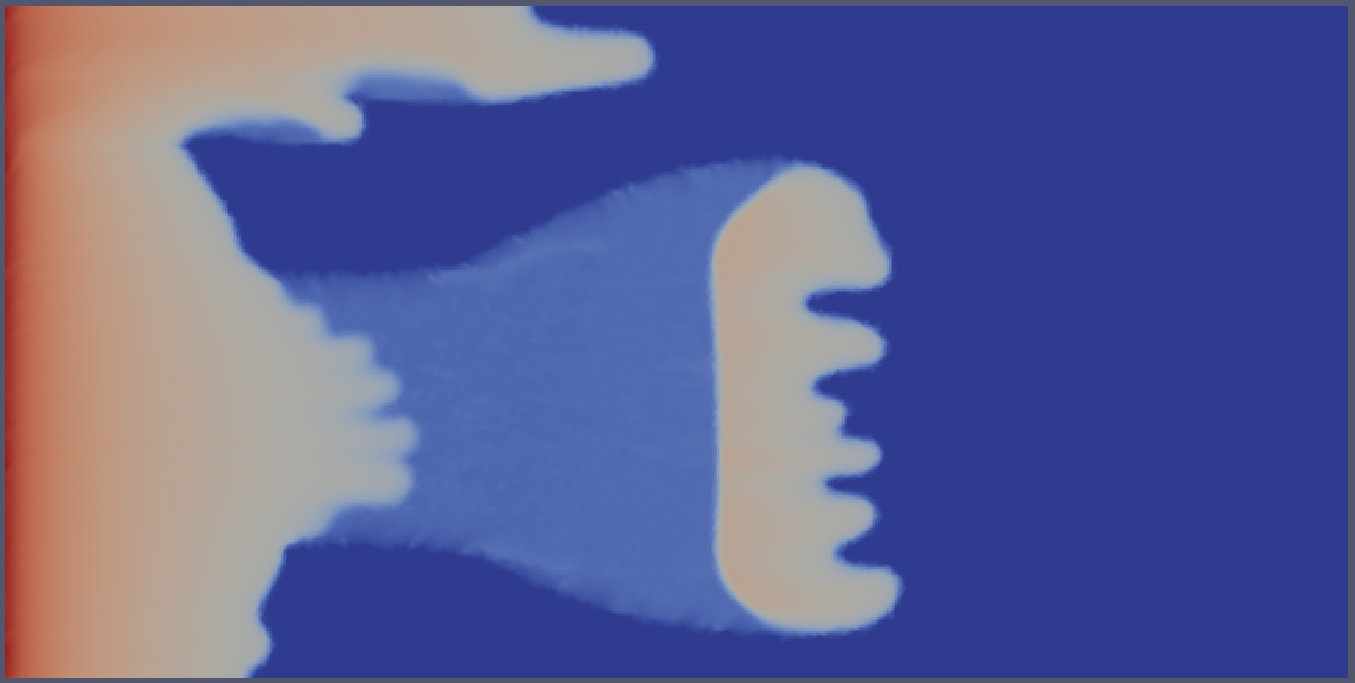
\includegraphics[width=.65\textwidth]{./Pics1/mr10_5regions_fixed/5regions_fixed_500.pdf} 
}
\vspace{0.0cm}
\hbox{\hspace{6.5cm} (a) flow at t=500 (fixed mesh)   
}
\vspace{0.25cm}
\hbox{\hspace{3.5cm}
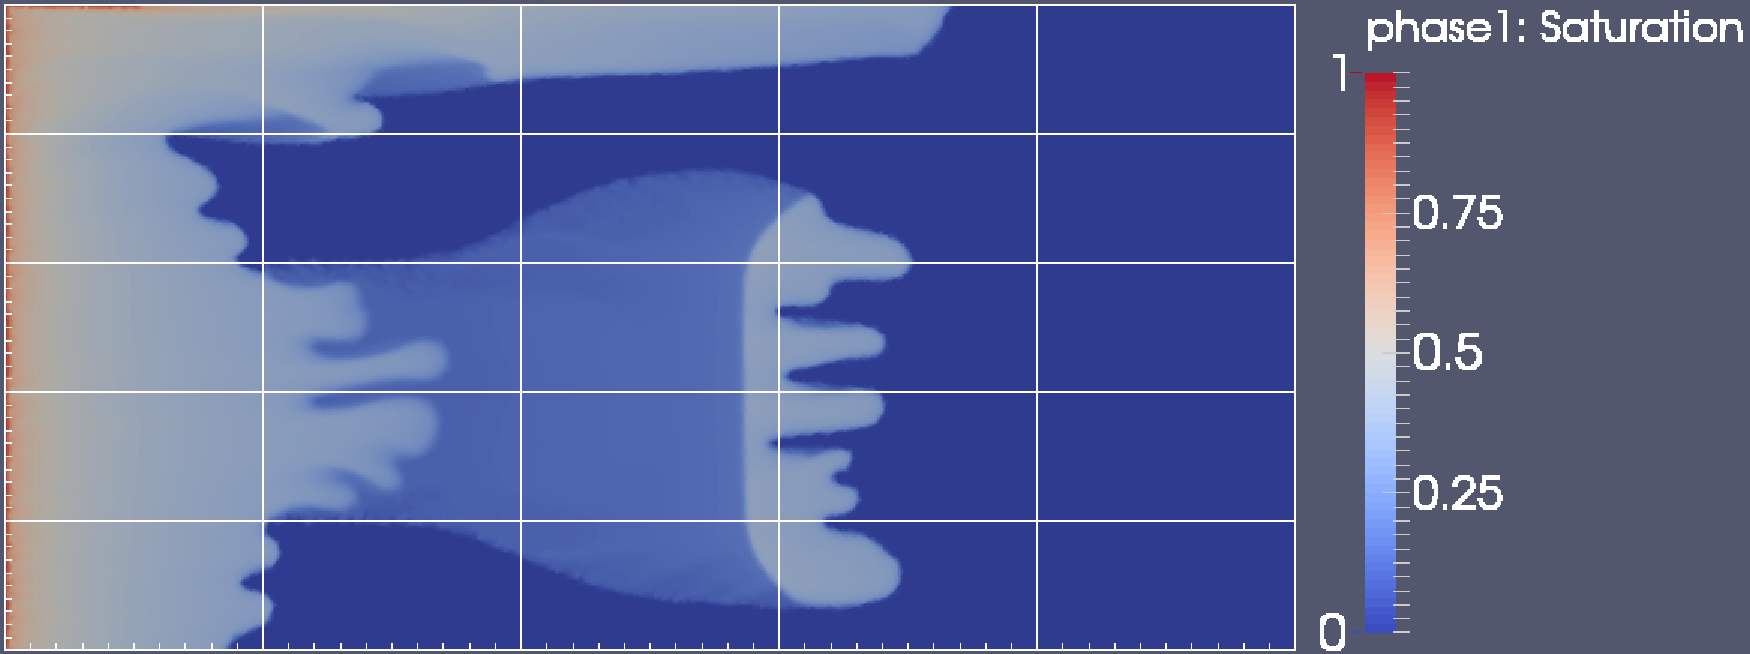
\includegraphics[width=.9\textwidth]{./Pics1/mr10_5regions_adapt/5regions_adapt_500_1.pdf}
}
\vspace{0.0cm}
\hbox{\hspace{6.5cm} (b) flow at t=500 (adaptive mesh)     
}
}     
\caption{At $t=0.25$s ($t=500$, timestemp) cross flow is taking place at the upper part of the formation. The fingers start to becoming more proufound as can been seen at the bottom.}
\label{fig:2testcase_b}
\end{figure}
\end{landscape}
\clearpage



%%%%
%%%%  FIGURE
%%%%
\begin{landscape}
\begin{figure}[ht] 
\vbox{
\hbox{\hspace{3.5cm}
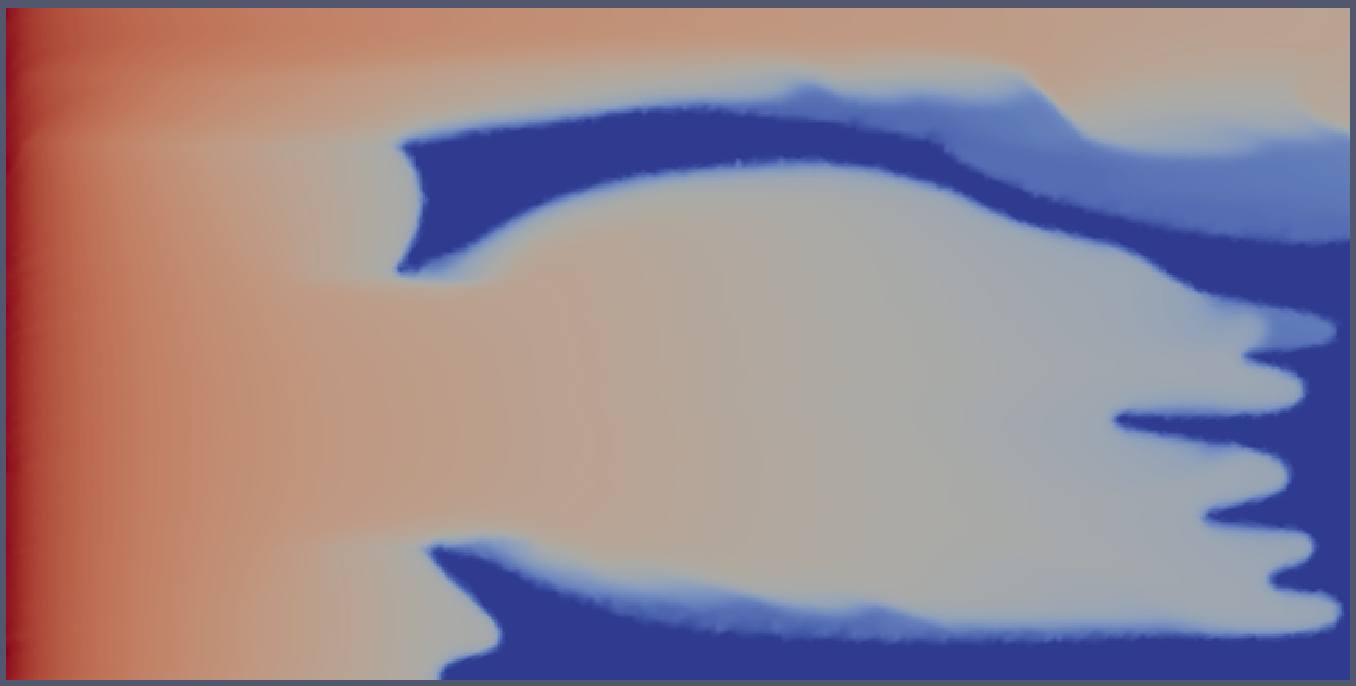
\includegraphics[width=.65\textwidth]{./Pics1/mr10_5regions_fixed/5regions_fixed_1500.pdf} 
}
\vspace{0.0cm}
\hbox{\hspace{6.5cm} (a) flow at t=1500 (fixed mesh)   
}
\vspace{0.25cm}
\hbox{\hspace{3.5cm}
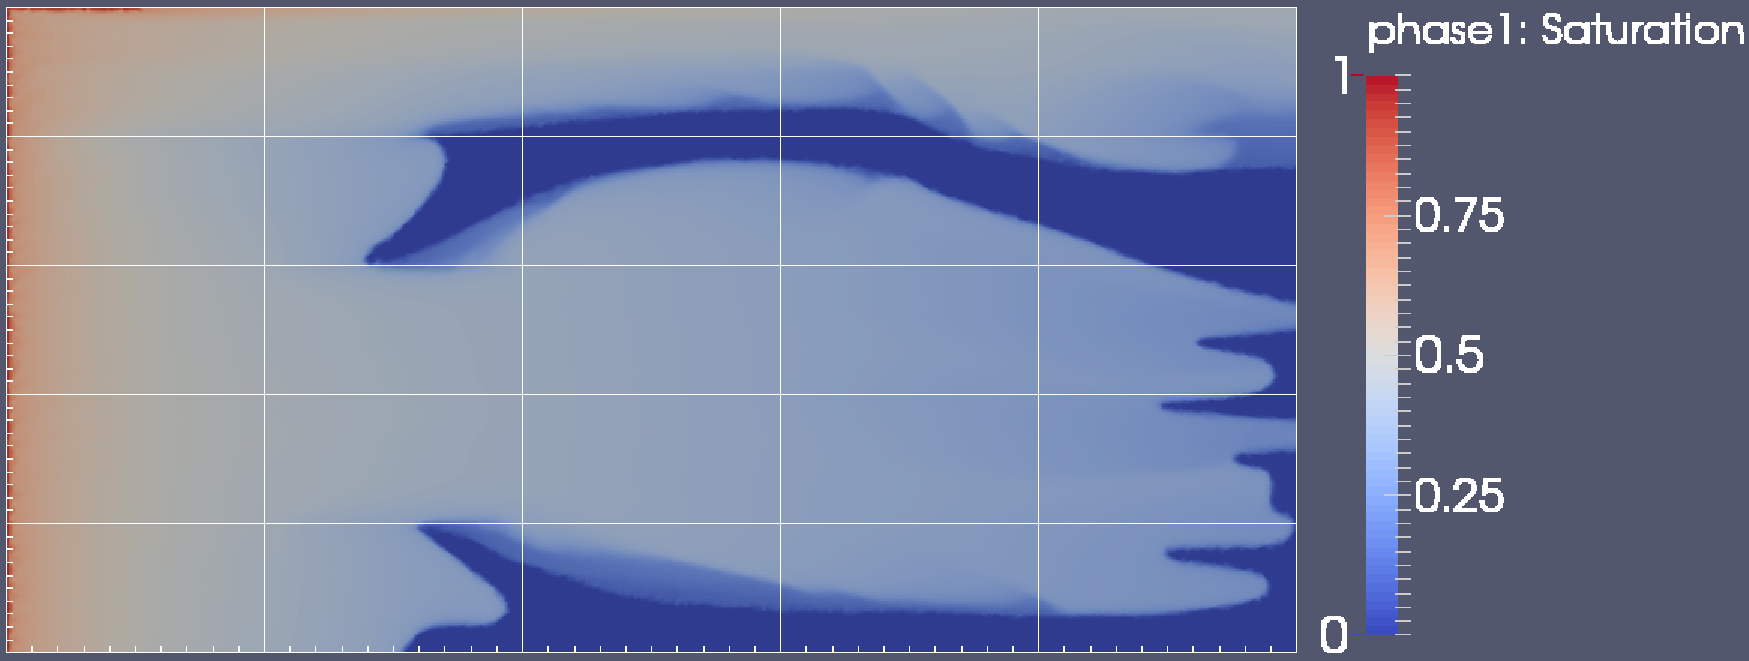
\includegraphics[width=.9\textwidth]{./Pics1/mr10_5regions_adapt/5regions_adapt_1500_1.pdf}
}
\vspace{0.0cm}
\hbox{\hspace{6.5cm} (b) flow at t=1500 (adaptive mesh)     
}
}     
\caption{At $t=0.75 sec$ ($t=1500$, timestemp) the initial cross flow is now fully developed and has travel all the way towards the outlet (right-hand side). and the finger below start forming a front that is also travelling towards the left-hand side.}
\label{fig:2testcase_c}
\end{figure}
\end{landscape}
\clearpage



%%%%
%%%%  FIGURE
%%%%
\begin{landscape}
\begin{figure}[ht] 
\vbox{
\hbox{\hspace{3.5cm}
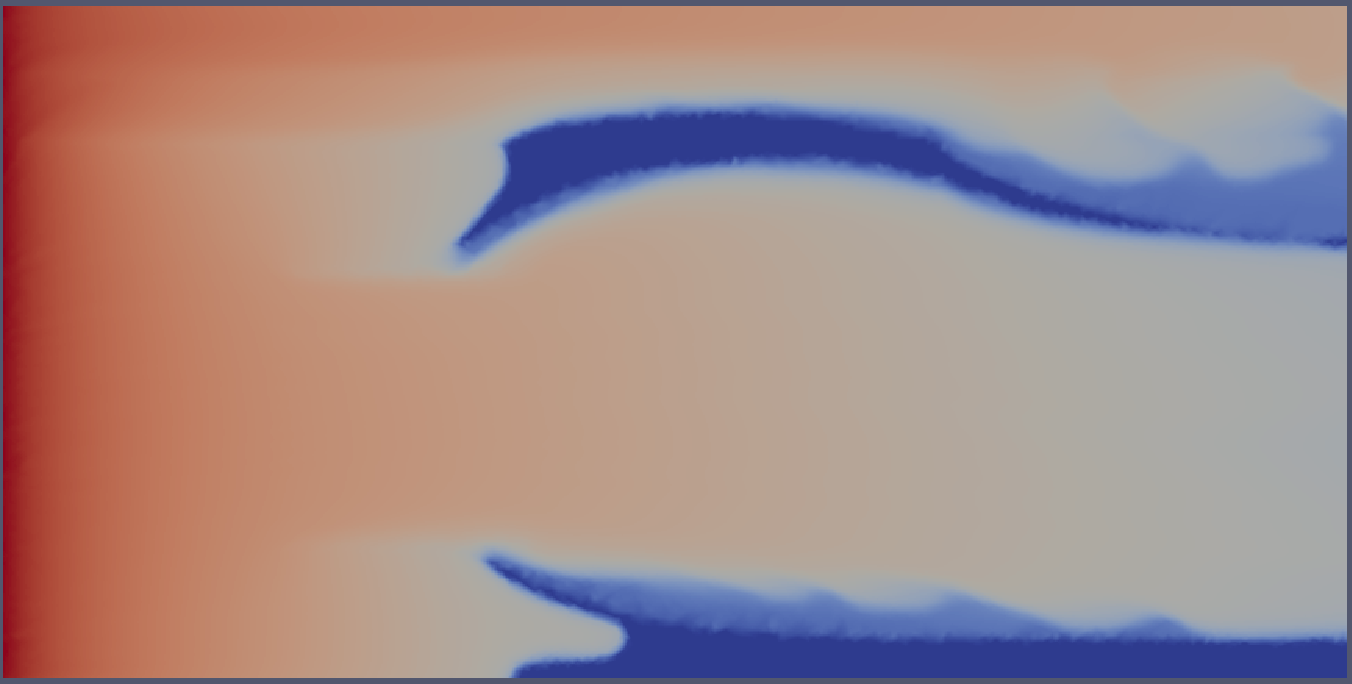
\includegraphics[width=.65\textwidth]{./Pics1/mr10_5regions_fixed/5regions_fixed_2000.pdf} 
}
\vspace{0.0cm}
\hbox{\hspace{6.5cm} (a) flow at t=end (fixed mesh)   
}
\vspace{0.25cm}
\hbox{\hspace{3.5cm}
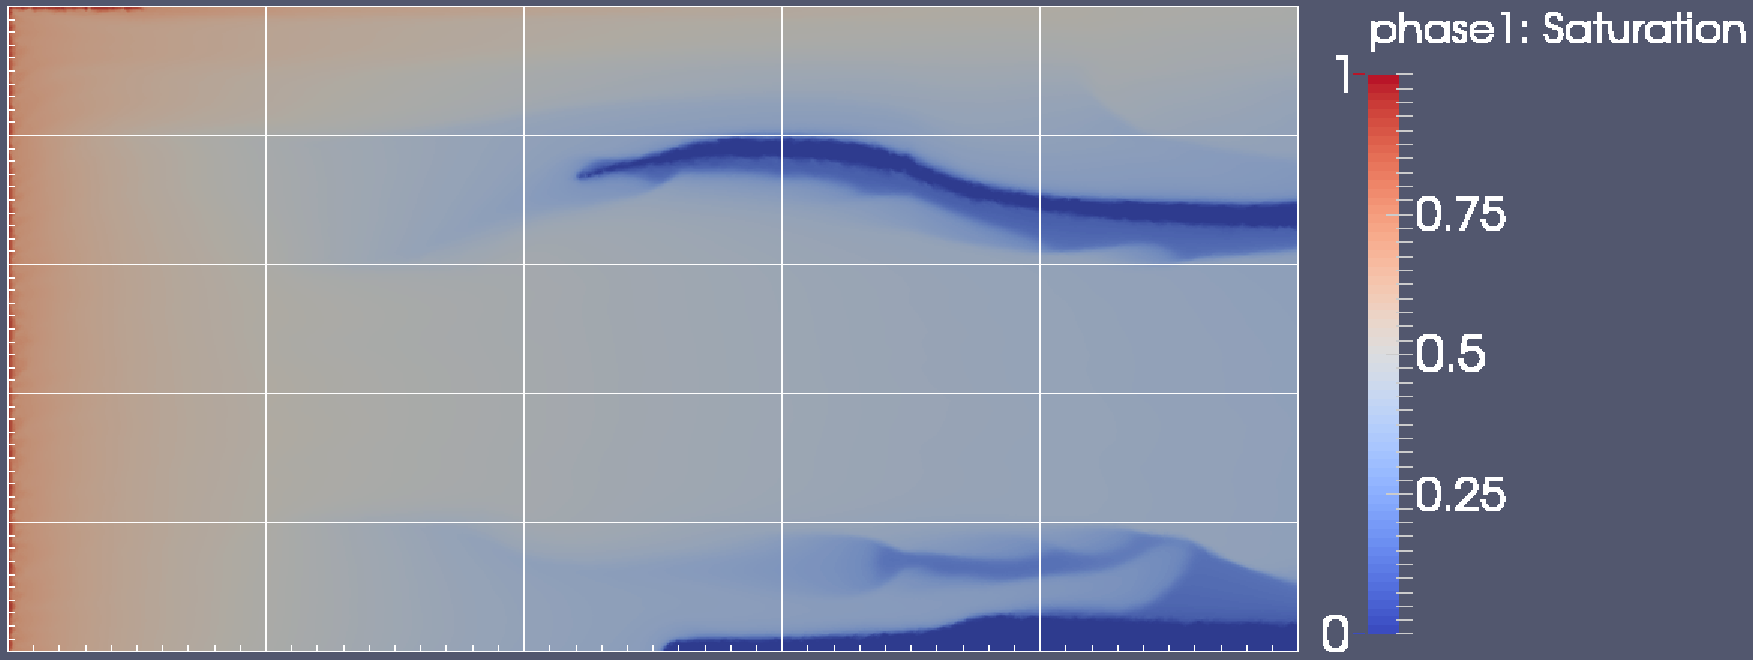
\includegraphics[width=.9\textwidth]{./Pics1/mr10_5regions_adapt/5regions_adapt_3000_1.pdf}
}
\vspace{0.0cm}
\hbox{\hspace{6.5cm} (b) flow at t=end (adaptive mesh)     
}
}     
\caption{Using the $P_{1}DGP_{2}$ element type for VR=$10$ under the same time steps, we compared the impact of fixed and adaptive mesh for the same timeframe. The end of simulation happens at $time=5 sec$ and for the timestemp $t=9999$ while the number of elements in both simulations was approximately $4700$. When adaptive mesh is introduce there is better repersentation of the fluid instabilities as these are developed on time.}
\label{fig:2testcase_d}
\end{figure}
\end{landscape}
\clearpage



%%%%
%%%%  FIGURE
%%%%
\begin{landscape}
\begin{figure}[ht] 
\vbox{
\hbox{\hspace{3.5cm}
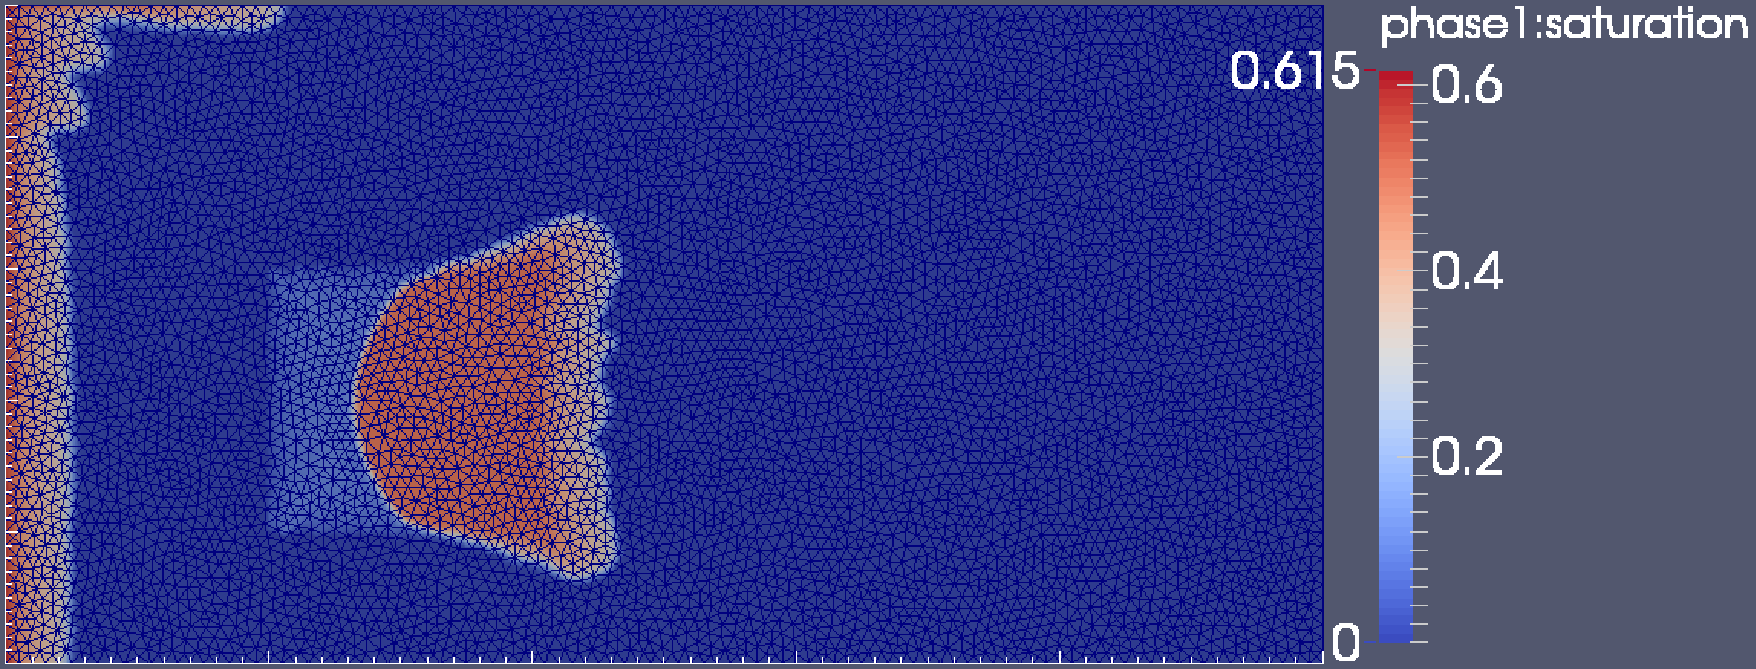
\includegraphics[width=.9\textwidth]{./Pics1/mr10_5regions_fixed_dinlet/5regions_dinlet_fixed_100_1.pdf}
}
\vspace{0.0cm}
\hbox{\hspace{6.5cm} (a) double inlet - fixed mesh   
}
\hbox{\hspace{3.5cm}
  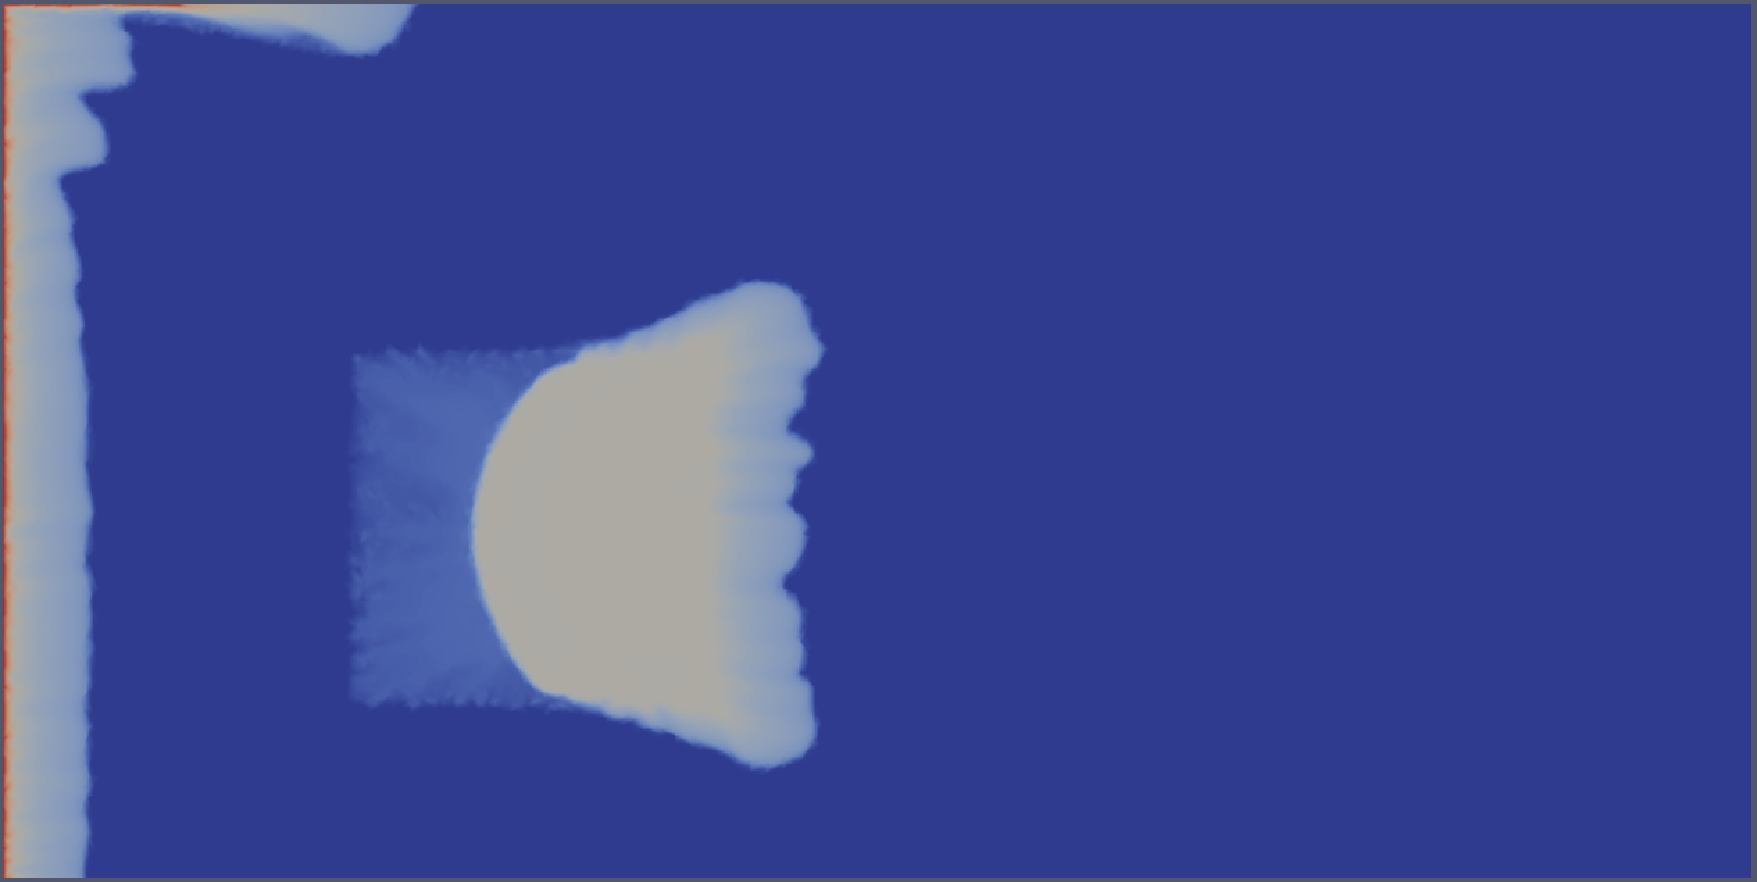
\includegraphics[width=.67\textwidth]{./Pics1/mr10_5regions_adapt_dinlet/5regions_dinlet_adapt_start.pdf}
}
\vspace{0.0cm}
\hbox{\hspace{6.5cm} (b) double inlet adaptive mesh   
}
}     
\caption{Comparing test-cases of fixed and adaptive mesh while a second region/inlet is introduced. For $t=0.101$s, using the $P_{1}DGP_{2}$ element type for MR=$10$ under the same time steps. For this simulation there are $13226$ elements for the fixed messh and $43716$ for the adaptive.}
\label{fig:3testcase_a}
\end{figure}
\end{landscape}
\clearpage

%%%%
%%%%  FIGURE
%%%%
\begin{figure}[ht] 
\vbox{
\hbox{\hspace{3.5cm}
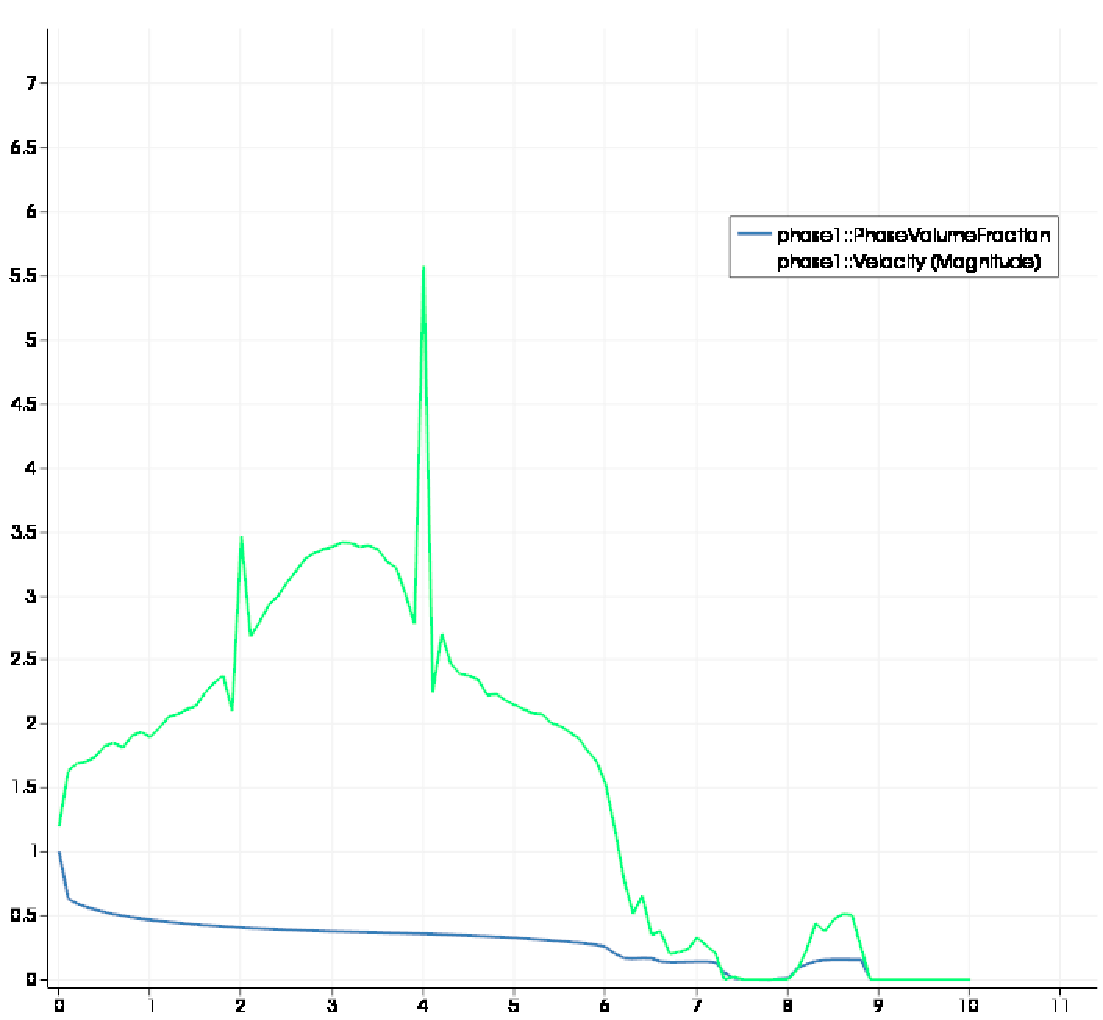
\includegraphics[width=.5\textwidth]{./Pics1/mr10_5regions_adapt/5regions_adapt_vel_magn.pdf} 
}
\vspace{0.0cm}
\hbox{\hspace{5.0cm} (a) single inlet velocity magnitude   
}
\hbox{\hspace{3.5cm}
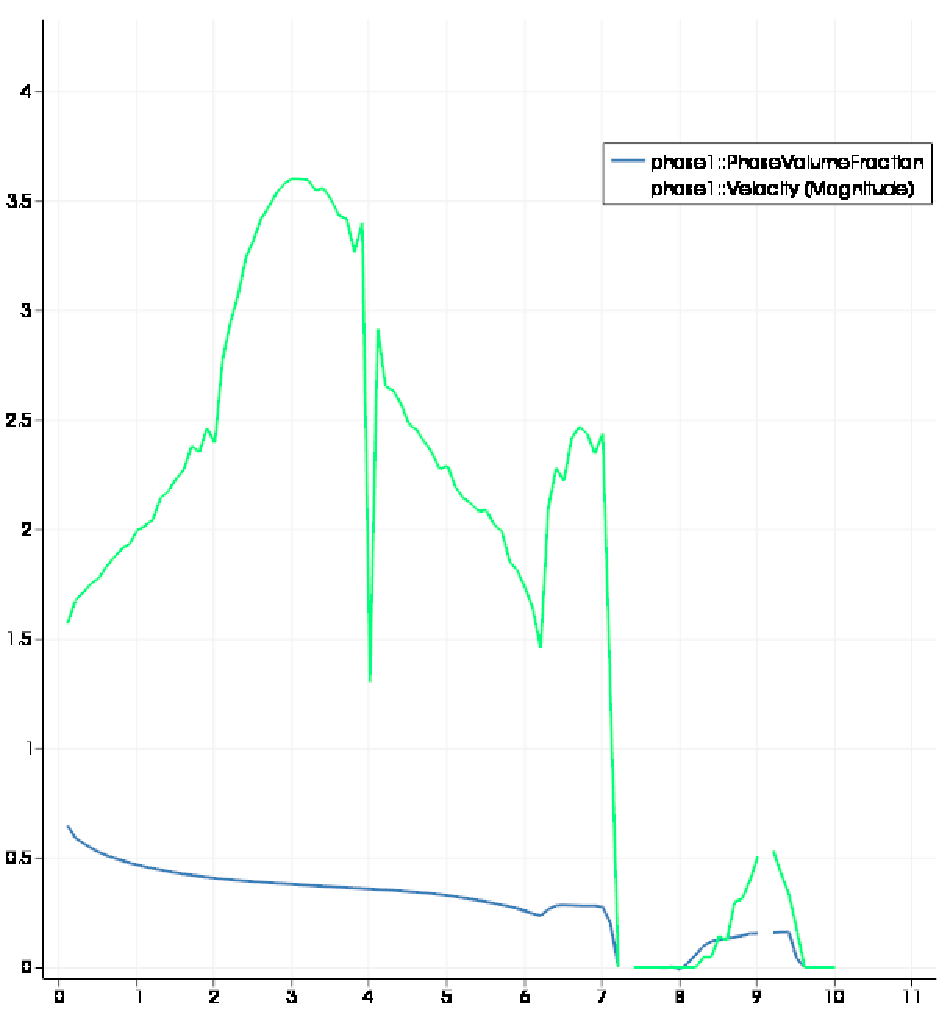
\includegraphics[width=.5\textwidth]{./Pics1/mr10_5regions_adapt_dinlet/5regions_dinlet_adapt_vel_magn.pdf}
}
\vspace{0.0cm}
\hbox{\hspace{5.0cm} (b) double inlet velocity magnitude   
}
}     
\caption{For the same time step, t=1000, these plots describe the velocity magnitudes of the phase $1$ (injected fluid) under the same boundary and initiall conditions. From top to bottom,these graphs describe the velocity magnitude %for fixed mesh is plotted(top), the velocity magnitude 
for adaptive mesh-single inlet (top) and the velocity magnitude for adaptive mesh with double inlet (bottom) as these are also presented in fig.\ref{fig:3testcase_a}. The main difference between the upper and lower plot %is not just the ability to capture in greater detail, the fluid instabilities as they happenduring the finger development and their velocity patterns. While there 
is the impact of the second injection interval as this can be seen from the slope and the rate that the velocity magnitude is changing.}
\label{fig:vel_magn}
\end{figure}

%%%%
%%%%  FIGURE
%%%%
\begin{landscape}
\begin{figure}[ht] 
\vbox{
\hbox{\hspace{3.5cm}
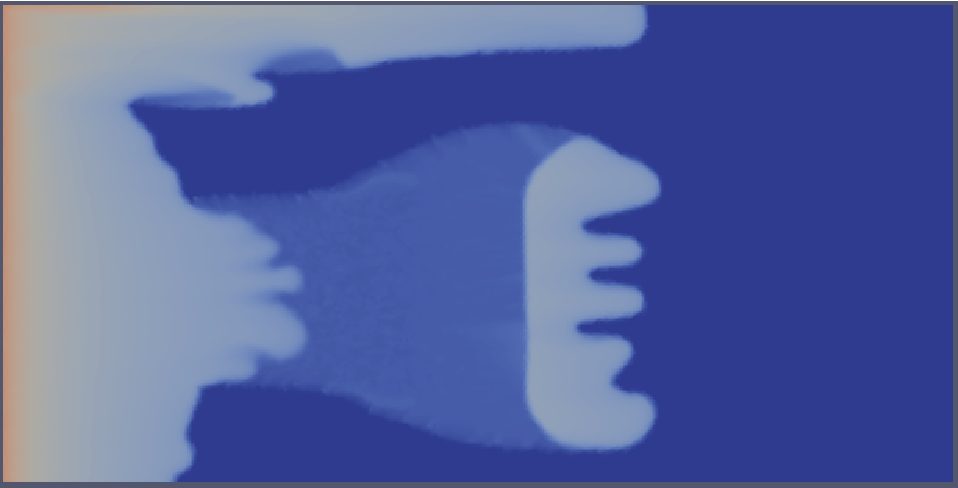
\includegraphics[width=.65\textwidth]{./Pics1/5reg_dinlet_fixed_500.pdf} 
}
\vspace{0.0cm}
\hbox{\hspace{6.5cm} (a) double inlet - fixed mesh   
}
\hbox{\hspace{3.5cm}
\includegraphics[width=.9\textwidth]{./Pics1/5reg_dinlet_adapt_500_1.pdf}
}
\vspace{0.0cm}
\hbox{\hspace{6.5cm} (b) double inlet adaptive mesh   
}
}     
\caption{For $t=5$s there is a comparison between fixed mesh(a) and adaptive mesh(b).}
\label{fig:3testcase_b}
\end{figure}
\end{landscape}
\clearpage

%%%%
%%%%  FIGURE
%%%%
\begin{landscape}
\begin{figure}[ht] 
\vbox{
\hbox{\hspace{3.5cm}
\includegraphics[width=.65\textwidth]{./Pics1/5reg_dinlet_fixed_1500.pdf} 
}
\vspace{0.0cm}
\hbox{\hspace{6.5cm} (a) double inlet - fixed mesh   
}
\hbox{\hspace{3.5cm}
\includegraphics[width=.9\textwidth]{./Pics1/5reg_dinlet_adapt_1500_1.pdf}
}
\vspace{0.0cm}
\hbox{\hspace{6.5cm} (b) double inlet adaptive mesh   
}
}     
\caption{For $t=7.5$s this is a comparison between fixed mesh(a) and adaptive mesh(b).}
\label{fig:3testcase_c}
\end{figure}
\end{landscape}
\clearpage

%%%%
%%%%  FIGURE
%%%%
\begin{landscape}
\begin{figure}[ht] 
\vbox{
\hbox{\hspace{3.5cm}
\includegraphics[width=.65\textwidth]{./Pics1/5reg_dinlet_fixed_end.pdf} 
}
\vspace{0.0cm}
\hbox{\hspace{6.5cm} (a) double inlet - fixed mesh   
}
\hbox{\hspace{3.5cm}
\includegraphics[width=.9\textwidth]{./Pics1/5reg_dinlet_adapt_end_1.pdf}
}
\vspace{0.0cm}
\hbox{\hspace{6.5cm} (b) double inlet adaptive mesh   
}
}     
\caption{This is a comparison between fixed mesh(a) and adaptive mesh(b) at the end of the simulation. For the fixed mesh at this point the maximum number of point is $13226$ while for the adaptive mesh is $7582$ and most of them are located where is needed in the domain.}
\label{fig:3testcase_d}
\end{figure}
\end{landscape}
\clearpage

%%%%
%%%%  FIGURE
%%%%
\begin{landscape}
\begin{figure}[ht] 
\vbox{
\hbox{\hspace{3.5cm}
\includegraphics[width=.8\textwidth]{./Pics1/mr100_fixed/mr100_fixed_500.pdf} 
}
\vspace{0.0cm}
\hbox{\hspace{4.0cm} (a) fixed and unstructured mesh for MR = 100 (start)   
}
\hbox{\hspace{3.5cm}
\includegraphics[width=.8\textwidth]{./Pics1/mr100_fixed/mr100_fixed_1500.pdf}
}
\vspace{0.0cm}
\hbox{\hspace{3.75cm} (b) fixed and unstructured mesh for MR = 100 (t = 1500)   
}
}     
\caption{For the case of VR=$100$ from top to bottom, the number of elements is $4680$ and fixed and unstructured mesh for the same time steps, t=$0.25$ or t=500(a), t=$0.75$ or t=1500(b). }
\label{fig:4testcase_a}
\end{figure}
\end{landscape}
\clearpage

%%%%
%%%%  FIGURE
%%%%
\begin{landscape}
\begin{figure}[ht] 
\vbox{
\hbox{\hspace{3.5cm}
\includegraphics[width=.8\textwidth]{./Pics1/mr100_fixed/mr100_fixed_3000.pdf} 
}
\vspace{0.0cm}
\hbox{\hspace{3.75cm} (c) fixed and unstructured mesh for MR = 100    
}
\hbox{\hspace{3.5cm}
\includegraphics[width=.8\textwidth]{./Pics1/mr100_fixed/mr100_fixed_end.pdf}
}
\vspace{0.0cm}
\hbox{\hspace{7.cm} (d) end of simulations     
}
}     
\caption{screenshot (c) is for t=$1.5$ sec or t=$3000$ and screenshot (d) is for t=$3.175$ sec, at the end of the simulations. }
\label{fig:4testcase_b}
\end{figure}
\end{landscape}
\clearpage



%

%%%
%%%  FIGURE 
%%%
\begin{figure}[h]
\begin{center}
\includegraphics[width=1.\textwidth]{diagrams/bl-exact-meth-upwind.eps}
\end{center}
\caption{Buckley--Leverett test-cases: Saturation solutions for the continuous upwind method for different 1D P$_{1}$DG-P$_{2}$ mesh  resolutions and comparison against standard analytical solution.
\label{bl-exact-meth-upwind}}
\end{figure}

%%%
%%%
%%%  FIGURE 
%%%
\begin{figure}[h]
  %\begin{center}
\vbox{\hbox{\hspace{2.5cm}
    \includegraphics[width=0.62\textwidth]{diagrams/BL_1d_P0DGP1_convergence.eps}}
\vspace{-.0cm}\hbox{\hspace{2.5cm}
    \includegraphics[width=0.62\textwidth]{diagrams/BL_1d_P1DGP2_convergence.eps}}
\vspace{-.0cm}\hbox{\hspace{2.5cm}
    \includegraphics[width=0.62\textwidth]{diagrams/BL_1d_P2DGP3_convergence.eps}}}
   % \includegraphics[width=0.45\textwidth]{BL_2d_P1DGP2_convergence}
    \caption{Buckley--Leverett test-cases: Saturation profiles for a number of element-pairs and numerical resolutions in 1D -- P$_{0}$DG-P$_{1}$ (top), P$_{1}$DG-P$_{2}$ and P$_{2}$DG-P$_{3}$ (bottom).\label{fig:BL_profiles}}
  %\end{center}
\end{figure}

%%%
%%%  FIGURE 
%%%
\begin{figure}[h]
\vbox{\hbox{\hspace{1.cm}
    \includegraphics[width=0.8\textwidth]{diagrams/L1_convergence_rate.eps}}
\vspace{.0cm}\hbox{\hspace{1.cm}
    \includegraphics[width=0.8\textwidth]{diagrams/L2_convergence_rate.eps}}}
    \caption{Buckley--Leverett test-cases: L1 (top) and L2 (bottom) error convergence rates for a number of element pairs. \label{fig:BL_converg-rates}}
\end{figure}

%%%
%%%  FIGURE 
%%%
\begin{figure}[h]
\begin{center}
\includegraphics[width=1.\textwidth]{diagrams/bl-upwind-v-up-and-down.eps}
\end{center}
\caption{Buckley--Leverett test-cases: Comparison of the optimal upwind formulation when using upwinding (OU) and coupled upwind/downwind (OU-D). The finite element interpolation of the saturation field $\left(S_{1}\right)$ is shown at different mesh resolutions. Downwind seems to detract from the accuracy of the solution. \label{bl-upwind-v-up-and-down}}
\end{figure}

%%%
%%%  FIGURE 
%%%
\begin{figure}[h]
\vbox{
\begin{center}
\includegraphics[width=1.\textwidth]{diagrams/bl-exact-meth-cv-0-8-ele50.eps}
\end{center}
\vspace{0.cm}}
\caption{Buckley--Leverett test-cases: Comparison of control volume
  solutions using 80$\%$ upwinding and with optimal upwinding and
  using 50 continuous P$_{1}$DG-P$_{2}$
  elements. \label{bl-exact-meth-cv-0-8-ele50}}
\end{figure}

%%%
%%%  FIGURE 
%%%
\begin{figure}[h]
\begin{center}
\includegraphics[width=1.\textwidth]{diagrams/bl-dg-2eles.eps}
\end{center}
\caption{Buckley--Leverett test-cases: Two element solution using the
  discontinuous formulation. Saturation field from both CV solution
  and FEM interpolation are shown.  \label{bl-dg-2eles}}
\end{figure}

%%%
%%%  FIGURE 
%%%
\begin{figure}[h]
\vbox{
\hbox{\hspace{.3cm}\includegraphics[width=.9\textwidth]{diagrams/bl-dg-4-10-20.eps}}
\vspace{-0.cm}
\hbox{\hspace{.3cm}\includegraphics[width=.9\textwidth]{diagrams/bl-dg-cent-4-10-20.eps}}}
\caption{Buckley--Leverett test-cases: Saturation field obtained from
  the discontinuous and continuous formulation with different mesh
  resolutions. Solutions with (top) and without (bottom) upwinding
  scheme. Notice that oscillations are suppressed with the upwinding
  scheme.\label{bl-dg-cent-4-10-20}}
\end{figure}


%%%
%%%  FIGURE 
%%%
\begin{figure}[h]
\vbox{
\hbox{\hspace{.3cm}\includegraphics[width=.9\textwidth]{diagrams/bl-dg-4-10-vers-cty.eps}}
\vspace{-0.cm}
\hbox{\hspace{.3cm}\includegraphics[width=.9\textwidth]{diagrams/bl-dg-p1-2-4-5-10-20-40.eps}}}
\caption{Buckley--Leverett test-cases: Saturation field obtained from
  (top) continuous and discontinuous (between elements) formulations
  (solution with 50 elements may be considered as a converged
  result). Solution obtained (bottom) from linear pressure (P1)
  formulation with different mesh resolution with comparison against
  P2-pressure formulation (continuous). \label{bl-dg-4-10-vers-cty}}
\end{figure}


%%%
%%%  FIGURE 
%%%
\begin{figure}[H]
\vbox{
\begin{center}
\includegraphics[width=17.5cm,height=12.5cm]{diagrams/bl-dg-4-10-vers-cty}
\end{center}
\vspace{0.cm}}
\caption{Gas saturations shown comparing the accuracy of the
  discontinuous between elements and continuous formulation. The 50
  element continuous solution may be viewed as a converged result.  }
\label{bl-dg-4-10-vers-cty}
\end{figure}

\begin{comment}
%%%
%%%  FIGURE 
%%%
\begin{figure}[h]
\vbox{
\hbox{\hspace{.2cm}
    \includegraphics[width=1.\textwidth]{diagrams/map_2d.png}}
\vspace{1.cm}
\hbox{\hspace{0.2cm}
    \includegraphics[width=1.\textwidth]{./diagrams/map_3d.png}}}
    \caption{Buckley-Leverett test-cases: phase 1 saturation surface maps for a 2- (770 triangles) and 3-D (1207 tetrahedra) simulations (\PN[1]{2} unstructured mesh grids) at time $t=0.5$. \label{fig:maps2d_3d}}
\end{figure}


%%%  FIGURE 
%%%
\begin{figure}[h]
\vbox{\hbox{\hspace{.3cm}
    \includegraphics[width=0.9\textwidth]{diagrams/BL_2d_P1DGP2_convergence.eps}}
\vspace{-.0cm}\hbox{\hspace{.3cm}
    \includegraphics[width=0.9\textwidth]{./diagrams/simulations_2d_3d.eps}}}
    \caption{Buckley-Leverett test-cases: 2- and 3-D phase 1 saturation profiles with \PN[1]{2} elements. Sensitivity analysis for (top) grid resolution using structured \PN[1]{2} mesh, and (bottom) mesh type.\label{fig:BL_2d_profiles}}
\end{figure}

\end{comment}



\end{document}

%%
%% End of tex file.
